% !TEX program = xelatex
% ============================================================================
% មគ្គុទ្ទេសក៍គរុកោសល្យគ្រូ និងសេណារីយ៉ូបង្រៀនលម្អិត (Teacher's Guideline -- EXP_MUL)
% មុខវិជ្ជា៖ គណិតវិទ្យា ថ្នាក់ទី៨ -- មេរៀនទី២៖ ស្វ័យគុណ
% ចំណុចរង៖ ២.២. វិធីគុណស្វ័យគុណមាននិទស្សន្តរ៉ឺឡាទីប (ទំ.១៥ និង ២៥)
% គ្រូបង្រៀន៖ ហុក ប៊ុនថែន | អនុវិទ្យាល័យព្រះក្រសាំង (កំពង់ស្វាយ-កំពង់ធំ)
% ============================================================================
\documentclass[a4paper,12pt]{article}

\usepackage[a4paper, left=1.45cm, right=1.45cm, top=2.30cm, bottom=2.30cm, headheight=18pt, headsep=0.68cm, footskip=0.88cm]{geometry}
\usepackage{amsmath, amssymb}
\usepackage{unicode-math}
\usepackage{fontspec}
\usepackage{array, longtable, multirow, colortbl, booktabs}
\usepackage[table]{xcolor}
\usepackage{enumitem}
\usepackage{pifont}
\usepackage{fancyhdr}
\usepackage{lastpage}
\usepackage{needspace}
\usepackage[hyphens]{url}
\usepackage{tikz}
\usepackage[most]{tcolorbox}
\tcbuselibrary{breakable,skins}
\usetikzlibrary{calc, arrows.meta, angles, quotes, decorations.markings, positioning, patterns, babel}
\urlstyle{same}

\makeatletter
\let\@expl@@@mark@update@singlecol@structures@@\relax
\makeatother

% ============================================================================
% ការកំណត់ពុម្ពអក្សរ (Cross-Platform Khmer + Times New Roman APA + Cambria Math)
% ============================================================================
\providecommand{\NGSFindFonts}{%
  \IfFileExists{C:/Windows/Fonts/cambria.ttc}{%
    \def\NGSSysPath{C:/Windows/Fonts/}%
    \def\NGSUserPath{C:/Users/KIT/AppData/Local/Microsoft/Windows/Fonts/}%
  }{%
    \IfFileExists{./fonts/KhmerOSsiemreap.ttf}{\def\NGSSysPath{./fonts/}\def\NGSUserPath{./fonts/}}{%
    \IfFileExists{../fonts/KhmerOSsiemreap.ttf}{\def\NGSSysPath{../fonts/}\def\NGSUserPath{../fonts/}}{%
    \IfFileExists{../../fonts/KhmerOSsiemreap.ttf}{\def\NGSSysPath{../../fonts/}\def\NGSUserPath{../../fonts/}}{%
    \IfFileExists{../../../fonts/KhmerOSsiemreap.ttf}{\def\NGSSysPath{../../../fonts/}\def\NGSUserPath{../../../fonts/}}{%
    \IfFileExists{../../../../fonts/KhmerOSsiemreap.ttf}{\def\NGSSysPath{../../../../fonts/}\def\NGSUserPath{../../../../fonts/}}{%
    \IfFileExists{../../../../../fonts/KhmerOSsiemreap.ttf}{\def\NGSSysPath{../../../../../fonts/}\def\NGSUserPath{../../../../../fonts/}}{%
    \IfFileExists{../../../../../../fonts/KhmerOSsiemreap.ttf}{\def\NGSSysPath{../../../../../../fonts/}\def\NGSUserPath{../../../../../../fonts/}}{%
      \def\NGSSysPath{../../../../../../../fonts/}\def\NGSUserPath{../../../../../../../fonts/}%
    }}}}}}}%
  }%
}
\NGSFindFonts

\setmathfont[
  Path={\NGSSysPath},
  FontIndex=1,
  Scale=1.06
]{cambria.ttc}

\defaultfontfeatures{Ligatures=TeX}

\setmainfont[
  Path={\NGSUserPath},
  Extension=.ttf,
  Script=Khmer,
  BoldFont={KhmerOSsiemreap},
  BoldFeatures={FakeBold=1.8},
  ItalicFont={KhmerOSsiemreap},
  ItalicFeatures={FakeSlant=0.25},
  BoldItalicFont={KhmerOSsiemreap},
  BoldItalicFeatures={FakeBold=1.8, FakeSlant=0.25}
]{KhmerOSsiemreap}

% ហាមដាក់ FakeBold លើ KhmerOSmuollight និងកុំរុំ \muol ក្នុង \textbf{...}
\newfontfamily\muol[
  Path={\NGSUserPath},
  Extension=.ttf,
  Script=Khmer
]{KhmerOSmuollight}

\newfontfamily\TimesEn[
  Path={\NGSSysPath},
  Extension=.ttf,
  Scale=1.02,
  BoldFont={timesbd},
  ItalicFont={timesi},
  BoldItalicFont={timesbi}
]{times}

\newfontfamily\Tacteing[
  Path={\NGSUserPath}
]{TACTENG.TTF}

\newfontfamily\CourierBullet[
  Path={\NGSSysPath},
  Extension=.ttf
]{cour}

% ក្បួនកាត់ពាក្យខ្មែរ (Khmer word wrapping)
\XeTeXlinebreaklocale "km"
\XeTeXlinebreakskip = 0pt plus 1pt minus 0.1pt

% Mobile-First comfortable line spacing (11.5pt / 18.2pt effective)
\linespread{1.22}

% ============================================================================
% ពណ៌ ស-ខ្មៅ (Strict Monochrome Grayscale Palette) & Fancyhdr
% ============================================================================
\definecolor{headgray}{HTML}{F2F2F2}
\definecolor{panelgray}{gray}{0.94}
\definecolor{stepgray}{HTML}{D9D9D9}
\definecolor{midgray}{gray}{0.82}
\definecolor{bordergray}{gray}{0.45}

\pagestyle{fancy}
\fancyhf{}
\renewcommand{\headrulewidth}{0.4pt}
\renewcommand{\footrulewidth}{0.4pt}
\fancyhead[L]{\rule[-3pt]{0pt}{14pt}\fontsize{9.5pt}{13pt}\selectfont មគ្គុទ្ទេសក៍គរុកោសល្យគ្រូ \en{(Grade 8 EXP\_MUL)}}
\fancyhead[R]{\rule[-3pt]{0pt}{14pt}\fontsize{9.5pt}{13pt}\selectfont មេរៀនទី២ \en{(}២.២\en{)}៖ វិធីគុណស្វ័យគុណមាននិទស្សន្តរ៉ឺឡាទីប}
\fancyfoot[L]{\rule{0pt}{13pt}\fontsize{9.5pt}{13pt}\selectfont កញ្ចប់ឯកសារ \en{NGS 5Es} \en{(}៥០ នាទី\en{)} \en{|} ហុក ប៊ុនថែន}
\fancyfoot[R]{\rule{0pt}{13pt}\fontsize{9.5pt}{13pt}\selectfont ទំព័រ \en{\thepage\ / \pageref{LastPage}}}

\fancypagestyle{firstpage}{%
  \fancyhf{}%
  \renewcommand{\headrulewidth}{0pt}%
  \renewcommand{\footrulewidth}{0.4pt}%
  \fancyfoot[L]{\rule{0pt}{13pt}\fontsize{9.5pt}{13pt}\selectfont កញ្ចប់ឯកសារ \en{NGS 5Es} \en{(}៥០ នាទី\en{)} \en{|} អនុវិទ្យាល័យព្រះក្រសាំង}%
  \fancyfoot[R]{\rule{0pt}{13pt}\fontsize{9.5pt}{13pt}\selectfont ទំព័រ \en{\thepage\ / \pageref{LastPage}}}%
}

\setlength{\parindent}{0pt}
\setlength{\parskip}{4.2pt}
\setlength{\tabcolsep}{4pt}
\setlength{\emergencystretch}{2em}
\setlist{itemsep=2.5pt, parsep=0pt}

% ============================================================================
% ម៉ាក្រូជំនួយ និងឋានានុក្រម \muol គ្មានតួអក្សរ ASCII បន្លំ
% ============================================================================
\newcommand{\en}[1]{{\TimesEn #1}}
\newcommand{\enbf}[1]{{\TimesEn\textbf{#1}}}
\newcommand{\enit}[1]{{\TimesEn\textit{#1}}}
\newcommand{\unit}[1]{\,\text{\en{#1}}}
\newcommand{\cnum}[1]{{\TimesEn\fontsize{10.5pt}{12pt}\selectfont\ding{\numexpr181+#1\relax}}}
\newcommand{\ditem}{\tikz[baseline=-0.5ex]\fill (0,0.40ex) -- (0.40ex,0) -- (0,-0.40ex) -- (-0.40ex,0) -- cycle;\hspace{0.25em}}
\newcommand{\wcirc}{{\CourierBullet\fontsize{9.8pt}{11pt}\selectfont o}}
\newcommand{\chkbox}{\tikz[baseline=-0.15ex]\draw[black, line width=0.85pt] (0,0) rectangle (0.25cm,0.25cm);}
\newcommand{\khmflourish}{{\Tacteing\fontsize{38pt}{15pt}\selectfont\raisebox{-5pt}{3}}}

\newcommand{\parttitle}[1]{{\muol\fontsize{14pt}{22pt}\selectfont #1}}
\newcommand{\sectitle}[1]{{\muol\fontsize{12pt}{19pt}\selectfont #1}}
\newcommand{\subsectitle}[1]{{\muol\fontsize{11.5pt}{18.5pt}\selectfont #1}}
\newcommand{\tblhead}[1]{{\muol\fontsize{10.2pt}{16pt}\selectfont #1\par}}
\newcommand{\callhead}[1]{{\muol\fontsize{11pt}{17pt}\selectfont #1}}
\newcommand{\scriptlead}{{\normalfont\mdseries\muol\fontsize{10.8pt}{17pt}\selectfont គ្រូនិយាយថា៖}}
\newcommand{\figcap}[2]{\vspace{3pt}{\fontsize{10.5pt}{16.5pt}\selectfont {\muol\fontsize{10.5pt}{16.5pt}\selectfont #1} #2}}

\newcolumntype{L}[1]{>{\raggedright\arraybackslash}p{#1}}
\newcolumntype{C}[1]{>{\centering\arraybackslash}p{#1}}
\newcolumntype{R}[1]{>{\raggedleft\arraybackslash}p{#1}}

\newcommand{\secbanner}[2]{%
  \Needspace{2.2cm}%
  \vspace{2pt}%
  \begin{tcolorbox}[
    enhanced, sharp corners, colback=stepgray, colframe=black,
    boxrule=1.1pt, borderline south={0.6pt}{1.8pt}{black},
    top=6pt, bottom=6pt, left=9pt, right=9pt,
    before skip=4pt, after skip=4pt
  ]
    \sectitle{#1}\\[2pt]
    {\fontsize{10pt}{14.5pt}\selectfont\enit{#2}}%
  \end{tcolorbox}%
}

\newcommand{\refbanner}[1]{%
  \Needspace{2.2cm}%
  \vspace{2pt}%
  \begin{tcolorbox}[
    enhanced, sharp corners, colback=headgray, colframe=black,
    boxrule=0.85pt, borderline south={0.6pt}{1.8pt}{black},
    top=6pt, bottom=6pt, left=9pt, right=9pt,
    before skip=4pt, after skip=4pt
  ]
    {\muol\fontsize{12pt}{19pt}\selectfont #1}%
  \end{tcolorbox}%
}

\newcommand{\subsec}[1]{%
  \Needspace{1.7cm}%
  \vspace{3pt}%
  \subsectitle{#1}\par%
  \vspace{-2pt}%
  {\color{black}\hrule height 0.55pt}%
  \vspace{3pt}%
}

\newtcolorbox{phasebox}[3]{%
  enhanced, breakable, sharp corners,
  colback=white, colframe=black,
  boxrule=1.0pt, top=5pt, bottom=5pt, left=9pt, right=9pt,
  toptitle=4pt, bottomtitle=4pt,
  before skip=5pt, after skip=0pt,
  colbacktitle=headgray, coltitle=black,
  fonttitle=\fontsize{11pt}{17.5pt}\selectfont,
  fontupper=\fontsize{11.5pt}{14.92pt}\selectfont,
  title={%
    \linespread{1.0}\selectfont\renewcommand{\arraystretch}{1.0}%
    \begin{tabular*}{\linewidth}{@{}>{\raggedright\arraybackslash}p{14.20cm}@{\extracolsep{\fill}}r@{}}
      {\muol\fontsize{11pt}{17.5pt}\selectfont #1} & {\fontsize{10.5pt}{14.5pt}\selectfont\en{#2 |} #3}%
    \end{tabular*}%
  }
}

\newtcolorbox{scriptbox}{%
  enhanced, breakable, sharp corners, colback=panelgray, colframe=black,
  boxrule=0.8pt, borderline west={2.4pt}{0pt}{black},
  top=5pt, bottom=5pt, left=9pt, right=9pt,
  before skip=-0.8pt, after skip=5pt,
  fontupper=\fontsize{11.5pt}{14.92pt}\selectfont
}

\begin{document}
\thispagestyle{firstpage}
\fontsize{11.5pt}{14.92pt}\selectfont
\vspace*{-0.75cm}

% ============================================================================
% ក្បាលលិខិតផ្លូវការថ្នាក់ជាតិ & សាលារៀន (Kampong Thom / Kampong Svay / Preah Krasang)
% ============================================================================
{\linespread{1.05}\selectfont
\begin{center}
  {\muol\fontsize{13.5pt}{21pt}\selectfont ព្រះរាជាណាចក្រកម្ពុជា}\\[2pt]
  {\muol\fontsize{12pt}{18.5pt}\selectfont ជាតិ សាសនា ព្រះមហាក្សត្រ}\\[1pt]
  \khmflourish
\end{center}
\vspace{-4pt}
{\muol\fontsize{10.8pt}{17pt}\selectfont
  មន្ទីរអប់រំ យុវជន និងកីឡា ខេត្តកំពង់ធំ\\
  ការិយាល័យអប់រំ យុវជន និងកីឡា ស្រុកកំពង់ស្វាយ\\
  អនុវិទ្យាល័យព្រះក្រសាំង\par}
\vspace{4pt}
\begin{center}
  \parttitle{មគ្គុទ្ទេសក៍គរុកោសល្យគ្រូ និងសេណារីយ៉ូបង្រៀនលម្អិត \enbf{(Teacher's Guideline)}}\\[3pt]
  {\fontsize{11.5pt}{18pt}\selectfont\textbf{មេរៀនទី២៖ ស្វ័យគុណ \en{---} ២.២. វិធីគុណស្វ័យគុណមាននិទស្សន្តរ៉ឺឡាទីប}}
\end{center}
}

\vspace{2pt}
\begin{tcolorbox}[
  enhanced, breakable, sharp corners, colback=headgray, colframe=black,
  boxrule=0.85pt, top=5pt, bottom=5pt, left=8pt, right=8pt,
  before skip=2pt, after skip=4pt
]
  \callhead{ព័ត៌មានរដ្ឋបាល និងឯកសារកញ្ចប់ \enbf{5} ផ្នែក}\par\vspace{2pt}
  \linespread{1.05}\fontsize{10.5pt}{14.8pt}\selectfont
  \renewcommand{\arraystretch}{1.15}
  \begin{tabular}{@{}L{3.10cm}@{}C{0.22cm}@{}L{5.10cm}@{\hspace{0.20cm}}L{2.70cm}@{}C{0.22cm}@{}L{5.50cm}@{}}
    \textbf{\en{-} មុខវិជ្ជា \en{/} ថ្នាក់} & \en{:} & គណិតវិទ្យា \en{(}ថ្នាក់ទី៨\en{)} & \textbf{\en{-} កាលបរិច្ឆេទ} & \en{:} & ថ្ងៃចន្ទ ទី១៦ ខែវិច្ឆិកា ឆ្នាំ២០២៦ \\
    \textbf{\en{-} ជំពូក \en{/} មេរៀន} & \en{:} & ពីជគណិត \en{/} មេរៀនទី២ ស្វ័យគុណ & \textbf{\en{-} រយៈពេល} & \en{:} & ៥០ នាទី \en{(}១ ម៉ោងសិក្សា\en{)} \\
    \textbf{\en{-} ចំណុចរង} & \en{:} & ២.២. វិធីគុណស្វ័យគុណមាននិទស្សន្តរ៉ឺឡាទីប & \textbf{\en{-} សៀវភៅគោល} & \en{:} & ទំ. ១៥ និង ២៥ \en{(\#6, \#7)} \\
    \textbf{\en{-} បង្រៀនដោយ} & \en{:} & ហុក ប៊ុនថែន & \textbf{\en{-} ឯកសារកញ្ចប់} & \en{:} & \en{4 Docs + 15 Verified OA PDFs}
  \end{tabular}
\end{tcolorbox}

% ============================================================================
% ផ្នែកទី ១៖ បរិបទមេរៀន ទិដ្ឋភាពកញ្ចប់ ៥ ផ្នែក និងកំណែសៀវភៅគោល
% ============================================================================
\secbanner{ផ្នែកទី ១៖ បរិបទមេរៀន ទិដ្ឋភាពកញ្ចប់ ៥ ផ្នែក និងកំណែសៀវភៅគោល}{Section 1: Administrative Context, 5-Part Lesson Package Overview, \& MoEYS Book pp. 15 \& 25 Errata}

\subsec{១\enbf{.}១ បរិបទអនុវិទ្យាល័យព្រះក្រសាំង និងតម្រូវការបង្រៀន ២\enbf{.}២}

មេរៀនរង \textbf{២.២. «វិធីគុណស្វ័យគុណមាននិទស្សន្តរ៉ឺឡាទីប»} ជាជំហានគន្លឹះភ្ជាប់ពីនិយមន័យ \textbf{២.១ ស្វ័យគុណនៃចំនួនសនិទានមាននិទស្សន្តជាចំនួនគត់} ($a^n$, $a^0=1$, $a^{-n}=\frac{1}{a^n}$ ទំ.១៤ និង ១៦) ឆ្ពោះទៅរកវិធានគុណ $a^m \cdot a^n = a^{m+n}$ សម្រាប់ $m, n \in \mathbb{Z}$ និងឯកធាតុពិជគណិតដូចជា $(-5xy^{-2})(\frac{3}{5}x^3y^8)$ ព្រមទាំងត្រៀមស្ពានទៅ \textbf{២.៣ វិធីចែកស្វ័យគុណ} (ទំ.១៦)។ ការវិភាគសៀវភៅគោលថ្នាក់ទី៨ ទំព័រ ១៥ និង ២៥ រួមជាមួយភស្តុតាងអន្តរជាតិចំនួន \en{15} អត្ថបទ បង្ហាញបញ្ហាប្រឈមស្នូល ៣ យ៉ាងនៅថ្នាក់ទី៨៖
\begin{itemize}[leftmargin=0.65cm]
  \item \textbf{១. អន្ទាក់ការយល់ច្រឡំលើនិទស្សន្តគត់រ៉ឺឡាទីប និងសញ្ញាដក៖} ការសិក្សាលើសិស្សថ្នាក់ទី៨បង្ហាញថា មានតែ \en{3.5\%} ប៉ុណ្ណោះដែលឆ្លើយត្រូវគ្រប់ ១០ សំណួរលើនិទស្សន្តរ៉ឺឡាទីប \en{(Ulusoy, 2019)} ដោយសិស្ស \en{59.4\%} ធ្វើខុសលើ $5^{-2}\cdot 5^4$ (គុណនិទស្សន្ត គុណគោល ឬទាញសញ្ញាដកទៅមុខ), \en{61.8\%} ខុសលើ $5^{-4}\cdot 6^4$ (គុណគោលផ្សេងគ្នា), និង \en{50\%} ភ្លេចសញ្ញាដកមុខឯកធាតុ \en{(Aydın-Güç \& Aygün, 2021)} ឬច្រឡំ $(-2)^4$ នឹង $-2^4$ \en{(Olson et al., 2011)}។
  \item \textbf{២. ការច្រឡំមេគុណ--អញ្ញាត និងអវត្តមាននិទស្សន្តលាក់ \en{1}៖} សិស្សតែងផ្ដោតលើលេខមុនអក្សរ \en{(47\%--59\%)} ឬយកច្បាប់គុណស្វ័យគុណទៅបូកអញ្ញាត \en{(Pournara et al., 2016)} ព្រមទាំងភ្លេចថា $x=x^1, y=y^1, 2=2^1$ ក្នុងលំហាត់ឯកធាតុ និងកិច្ចការផ្ទះ។
  \item \textbf{៣. កំណែកំហុសបោះពុម្ពសៀវភៅគោល (\en{MoEYS pp. 15, 25}) ទាំង ៣ ចំណុច៖} (i) \textbf{\en{Erratum \#1} (ប្រតិបត្តិ គ., ទំ.១៥)} បោះពុម្ពខុស $(3x^4 y^{-3})\allowbreak(-\frac{4}{3}x^{-2y})$ ដោយលោត $y$ ចូលនិទស្សន្ត $\to$ ត្រូវកែជា \textbf{$(3x^4 y^{-3})\allowbreak(-\frac{4}{3}x^{-2}y)$}; (ii) \textbf{\en{Erratum \#2} (ប្រអប់ ជាទូទៅ, ទំ.១៥)} ភ្លេចលក្ខខណ្ឌការពារ \textbf{$a \neq 0$} កាលណានិទស្សន្ត $\le 0$ ($0^0, 0^{-n}$ គ្មានន័យ) និងកំណត់ $m, n \neq 0$ ទាំងដែល ប្រតិបត្តិ ខ. បង្កើត $(-\frac{3}{2})^0 = 1$; (iii) \textbf{ទំ.២៥ \en{\#7} ក.} បោះពុម្ពខ្វះតួគុណទី២ ដូច្នេះត្រូវជៀសវាង ហើយដាក់តែ \textbf{\en{\#6} ក, ខ, គ និង \en{\#7} ខ} (ចៀសវាង \en{\#6} ឃ ដែលជាមេរៀនបន្ទាប់)។
\end{itemize}

មគ្គុទ្ទេសក៍នេះរចនាសកម្មភាពបែប \textbf{«វិស្វករសាងសង់ និងគ្រប់គ្រងម៉ាស៊ីនមេទិន្នន័យ (\en{Server Data Engineers})»} ក្នុងបរិបទឃ្លាំងវីដេអូឌីជីថលអនុវិទ្យាល័យព្រះក្រសាំង ($2^3 \times 2^4$ វីដេអូ និង $10^{-3} \times 10^4\unit{MB}$) ផ្សំជាមួយបន្ទះកត្តា ស-ខ្មៅ ខ្នាត \en{1:1} \en{(Guliman \& Alegre, 2021)}, ផ្ទាំងបន្សាបគូសូន្យ \en{(Rini, 2022)}, \en{Dual POE 2A--2B} \en{(Gustina et al., 2023; Maharani \& Subanji, 2018)}, ការអូសម្រាមដៃ \en{[tracing]} \en{(Yeo \& Tzeng, 2019)}, និងធនាគារហេតុផល \cnum{1}--\cnum{5} \en{(Wang et al., 2026; Wesenberg et al., 2022)}។

\subsec{១\enbf{.}២ កញ្ចប់ឯកសារ ៥ ផ្នែក និងផែនទីស៊ីចង្វាក់ ៥០ នាទី \enbf{(2 + 9 + 17 + 20 + $\le$2 min)}}

កញ្ចប់មេរៀន \en{EXP\_MUL} មានឯកសារ \en{LaTeX/PDF} ចំនួន ៤ គឺ \en{LS\_\allowbreak Plan\_\allowbreak EXP\_\allowbreak MUL}, \en{Teaching\_\allowbreak Scenario\_\allowbreak EXP\_\allowbreak MUL}, \en{Teaching\_\allowbreak Guideline\_\allowbreak EXP\_\allowbreak MUL}, និង \en{Printable\_\allowbreak Materials\_\allowbreak EXP\_\allowbreak MUL} (ទំព័រ ១--៦) រួមជាមួយថត ឯកសារស្រាវជ្រាវយោង\en{\_\allowbreak PDF} ដែលផ្ទុកឯកសារ \en{Open-Access} ចំនួន \en{15} ច្បាប់ និង \en{00\_\allowbreak}បញ្ជីឯកសារភស្តុតាង\en{\_\allowbreak Evidence\_\allowbreak Index.md} ផ្ទៀងផ្ទាត់ \en{SHA-256} ដូចគ្នា ១០០\% នឹងថត \en{03\_\allowbreak}ឯកសារស្រាវជ្រាវ៖

\begingroup
\linespread{1.0}\fontsize{10.2pt}{15.5pt}\selectfont
\renewcommand{\arraystretch}{1.28}
\begin{longtable}{|C{2.35cm}|L{3.45cm}|L{8.65cm}|C{2.40cm}|}
\hline
\rowcolor{headgray}
\multicolumn{1}{|C{2.35cm}|}{\tblhead{ជំហាន \enbf{/} ពេល}} &
\multicolumn{1}{C{3.45cm}|}{\tblhead{ឈ្មោះសកម្មភាព}} &
\multicolumn{1}{C{8.65cm}|}{\tblhead{ខ្លឹមសារស្នូល និងការតភ្ជាប់តាមឯកសារទាំង ៥}} &
\multicolumn{1}{C{2.40cm}|}{\tblhead{ទំព័របោះពុម្ព}} \\
\hline
\endfirsthead
\hline
\rowcolor{headgray}
\multicolumn{1}{|C{2.35cm}|}{\tblhead{ជំហាន \enbf{/} ពេល}} &
\multicolumn{1}{C{3.45cm}|}{\tblhead{ឈ្មោះសកម្មភាព}} &
\multicolumn{1}{C{8.65cm}|}{\tblhead{ខ្លឹមសារស្នូល និងការតភ្ជាប់តាមឯកសារទាំង ៥}} &
\multicolumn{1}{C{2.40cm}|}{\tblhead{ទំព័របោះពុម្ព}} \\
\hline
\endhead
\hline
\endfoot
\hline
\endlastfoot
\textbf{ជំហាន ១} \newline \en{00--02 min (2')} & រដ្ឋបាលថ្នាក់ & ពិនិត្យអវត្តមាន ចាត់ក្រុម ៣ នាក់ «វិស្វករម៉ាស៊ីនមេ» និងចែកទំព័រ ១ ផ្កាប់លើតុដើម្បីបង្ការការរំខានចក្ខុមុន \en{E1}។ & ទំព័រ ១ \en{(}ផ្កាប់\en{)} \\
\hline
\textbf{ជំហាន ២ក} \newline \en{02--05 min (3')} & កែកិច្ចការផ្ទះ \en{2.1} & ផ្ទៀងខ្លីទំ.១៤ ប្រតិបត្តិ \en{2} គ. $(-2)^7=-128$ និងទំ.២៥ \en{\#1} ខ. $(-8)^6$ (ញែកស្វ័យគុណគូ/សេសលើគោលដក)។ & ក្តារខៀន \\
\hline
\textbf{ជំហាន ២ខ} \newline \en{05--08 min (3')} & រំលឹកស្ពានមេរៀន & និយមន័យ $a^n$, បូកចំនួនគត់ $(-3+4=1,\; -2+8=6,\; -3+1=-2)$, លំនាំ $10^2\to 10^1\to 10^0=1\to 10^{-3}=\frac{1}{10^3}$ ($a\neq 0$), និងនិទស្សន្តលាក់ \en{1} ($x=x^1$)។ & ក្តារខៀន \\
\hline
\textbf{ជំហាន ២គ \en{(E1)}} \newline \en{08--11 min (3')} & បេសកកម្មឃ្លាំងវីដេអូ \en{Server} & ម៉ាស៊ីនមេអនុវិទ្យាល័យព្រះក្រសាំងមាន $2^3$ ថត $\times$ $2^4$ វីដេអូ និងឯកសារ $10^{-3}\times 10^4\unit{MB}$៖ ទស្សន៍ទាយ $2^7$ \en{vs} $4^7$ \en{vs} $2^{12}$ (មិនទាន់លាតចម្លើយ)។ & ក្តារខៀន \\
\hline
\textbf{ជំហាន ៣ក \en{(E2)}} \newline \en{11--22 min (11')} & បន្ទះ \en{1:1 (6')} \& \en{Dual POE (5')} & \textbf{ស.១}៖ ក្រិត $5.00\unit{cm}$, តបន្ទះ $2^3$ ($3.00\unit{cm}$) + $2^4$ ($4.00\unit{cm}$) $=7.00\unit{cm}$ ($2^7$), ផ្ទាំងបន្សាបគូសូន្យ $10^{-3}\times 10^4=10^1$; \textbf{ស.២}៖ \en{POE 2A} ($2^3\cdot 2^4\neq 4^7,\; 2^3\cdot 3^2\neq 6^5$) \& \en{POE 2B} ($3^2\cdot 3^3\neq 3^6,\; a\cdot a^3=a^4\neq a^3$)។ & ទំព័រ ១ \en{(1:1)} \\
\hline
\textbf{ជំហាន ៣ខ \en{(E3)}} \newline \en{22--28 min (6')} & បង្គុំច្បាប់ \en{\&} ធនាគារ \cnum{1}--\cnum{5} & សិស្សបង្គុំច្បាប់ពី ឧ. ក--ឃ (ទំ.១៥) មុនគ្រូ; កែ \textbf{\en{Erratum \#2}} ($a\neq 0$ កាលណា $m,n\le 0$) + ស្ពាន $a^{-n}=\frac{1}{a^n}, a^0=1$; តារាងសម្មតិកម្ម--សន្និដ្ឋាន--វិបាក និងផ្ទាំង \cnum{1}--\cnum{5}។ & ទំព័រ ៤ \en{(Poster)} \\
\hline
\textbf{ជំហាន ៤ក \en{(E4)}} \newline \en{28--38 min (10')} & កាត \en{[tracing]} លំហាត់គំរូ & ចែក \en{P2 (2-up)}: ដោះស្រាយ គំរូ ក, ខ, គ ទំ.១៥ ($10^{-3}\cdot 10^4=10$; $-35y^{10}$; $-3x^4y^6$) ដោយព័ទ្ធមេគុណ គូស \en{|} ក្រោម $x$, \en{||} ក្រោម $y$, ធ្នូនិទស្សន្ត + \en{EIA Looking-Back}។ & ទំព័រ ២ \en{(2-up)} \\
\hline
\textbf{ជំហាន ៤ខ \en{(E5)}} \newline \en{38--48 min (10')} & \en{Relay} ៣ តួនាទី \en{\& Exit A--D} & \textbf{ប្រតិបត្តិ ក, ខ, គ} (ទំ.១៥, កែ \textbf{\en{Erratum \#1}} $x^{-2y}\to x^{-2}y$: $x^{13},\; 1,\; -4x^2y^{-2}$) + បិទ \en{E1} ($128$ វីដេអូ, $10\unit{MB}$); កាតវិនិច្ឆ័យ \en{A--D} + សំបុត្រចេញ ៣ សំណួរ (៦០--៩០ វិនាទី)។ & ទំព័រ ៣ \en{\&} ទំព័រ ៥ \\
\hline
\textbf{ជំហាន ៥} \newline \en{48--50 min ($\le$2')} & កិច្ចការផ្ទះ \en{\&} ស្ពាន \en{2.3} & ចែក \en{P6} ទំ.២៥៖ \textbf{\en{\#6} ក, ខ, គ} និង \textbf{\en{\#7} ខ} (ជៀសវាង \en{\#7} ក បោះពុម្ពខ្វះតួ និង \en{\#6} ឃ) + ស្ពាន $2^7\cdot 2^{-4}$ \en{vs} $\frac{2^7}{2^4}$ ត្រៀមអាន \textbf{២.៣} (ទំ.១៦)។ & ទំព័រ ៦ \en{(Slips)} \\
\hline
\end{longtable}
\endgroup

% ============================================================================
% ផ្នែកទី ២៖ ការសំយោគឯកសារស្រាវជ្រាវអន្តរជាតិ (Mini-Literature Review)
% ============================================================================
\secbanner{ផ្នែកទី ២៖ ការសំយោគឯកសារស្រាវជ្រាវអន្តរជាតិ \enbf{(Mini-Literature Review)}}{Section 2: Research-to-Practice Synthesis Grounded in All 15 Verified Open-Access Studies}

\subsec{២\enbf{.}១ មុំទី១៖ ការយល់ច្រឡំ និងឧបសគ្គការគិតលើនិទស្សន្តរ៉ឺឡាទីប និងឯកធាតុ}

ការសិក្សាអំពីការយល់ដឹងរបស់សិស្សថ្នាក់ទី៨លើស្វ័យគុណមាននិទស្សន្តគត់រ៉ឺឡាទីបបង្ហាញពីអត្រាកំហុសធ្ងន់ធ្ងរ និងស្មុគស្មាញ។ ក្នុងការវាយតម្លៃសិស្សថ្នាក់ទី៨ \en{N = 165} នាក់ (អាយុ ១៣--១៤ ឆ្នាំ, ១០ សំណួរសរសេរ + សម្ភាសន៍ \en{n = 12}) \en{Ulusoy (2019, pp. 58--64)} រកឃើញថា មានសិស្សតែ \en{4} នាក់ (\en{3.5\%}) ប៉ុណ្ណោះឆ្លើយត្រូវគ្រប់សំណួរ ហើយជាង \en{65\%} ទទួលបានពិន្ទុក្រោម \en{3/10}។ ជាក់ស្ដែងលើវិធីគុណគោលដូចគ្នា \en{Q6} ($5^{-2}\cdot 5^4$, ខុស \en{59.4\%}) សិស្ស \en{8.4\%} (\en{n = 14}) គុណនិទស្សន្តជំនួសការបូក ($5^{-8}$/$5^8$), \en{3\%} (\en{n = 5}) គុណគោល ($25^{\pm 2}$/$25^{\pm 6}$), \en{3\%} គុណទាំងគោលទាំងនិទស្សន្ត ($25^{-8}$), \en{16.5\%} លុបសញ្ញាដកចោលព្រោះនិទស្សន្តគូ និង \en{16\%} រំកិលសញ្ញាដកទៅមុខគោល ($-5^2\cdot 5^4$)។ រីឯលើគោលខុសគ្នា \en{Q7} ($5^{-4}\cdot 6^4$, ខុស \en{61.8\%}) សិស្ស \en{16.9\%} (\en{n = 28}) គុណគោល ($30^{-4}$/$30^4$), \en{7.8\%} (\en{n = 13}) គុណគោលហើយបូកនិទស្សន្ត ($30^0$/$30^{\pm 8}$), \en{3\%} បូកទាំងគោលទាំងនិទស្សន្ត ($11^0$) និង \en{20\%} ទាញសញ្ញាដកទៅមុខគោល។ លើសពីនេះ លើនិទស្សន្តសូន្យ \en{Q1} ($-3^0$, ខុស \en{66.1\%}, ទទេ \en{11.5\%}) សិស្ស \en{30.9\%} (\en{n = 51}) សន្មតខុសថា $-3^0 = (-3)^0 = 1$, \en{14.5\%} (\en{n = 24}) គិតថានិទស្សន្តសូន្យស្មើនឹងការបូកសូន្យ ($-3^0 = -3$) និង \en{6.6\%} គិតថាស្មើ $0$; លើ \en{Q2} ($2^{-4}$, ខុស \en{63.6\%}) សិស្ស \en{23.6\%} (\en{n = 39}) សរសេរ $-2^4 = -16$ និង \en{13.9\%} លុបដកចេញ ($16$); ខណៈ \en{4\%} (\en{n = 7}) គុណគោលនឹងនិទស្សន្ត ($2^4 = 8$) និង \en{18.1\%--24.8\%} យកច្បាប់បូកនិទស្សន្តទៅអនុវត្តខុសលើផលបូក។

បន្ថែមពីនេះ កំហុសលើសញ្ញាដក វង់ក្រចក និងឯកធាតុពិជគណិតបង្ហាញភាពស្អិតរមួតខ្លាំង។ \en{Olson et al. (2011, pp. 117--118)} បានពិសោធន៍លើនិស្សិត \en{N = 904} នាក់ និងសម្ភាសន៍ \en{n = 19} នាក់ ហើយរកឃើញថា មានតែ \en{5/19} នាក់ប៉ុណ្ណោះប្រៀបធៀប $(-17)^8$ និង $-17^8$ បានត្រឹមត្រូវ ដោយ \en{6} នាក់អះអាងថា \en{«Parentheses don't matter»} ព្រោះស្អិតភ្ជាប់សញ្ញាដកជាមួយគោលជាជាងគិតជា $-1 \times 17^8$ ហើយភាពរឹងស្ដួចនៃសញ្ញាផ្ទុយនេះរារាំងការយល់ $n^{-1}$ ជាចម្រាសគុណ។ ក្នុងកម្រិតថ្នាក់ទី៨ផ្ទាល់ \en{Aydın-Güç \& Aygün (2021, pp. 1116--1118)} លើសិស្ស \en{N = 48} នាក់ (ស្រី \en{24}, ប្រុស \en{24}) រកឃើញថា \en{50\%} (\en{n = 24}) ព្រងើយកន្តើយចោលសញ្ញាដកមុខឯកធាតុ (ដូចសិស្ស S23 និយាយថា \en{«No need to pay attention to them»}), \en{25\%} (\en{n = 12}) បំបែកពន្លាតខុស, \en{38\%} (\en{n = 18}) អនុវត្តប្រមាណវិធីម្ខាងទៅម្ខាងទៀតខុស និង \en{29\%} បកប្រែលំដាប់ខុស។ ទន្ទឹមគ្នា \en{Pournara et al. (2016, Tables 2--4)} តាមដានសិស្ស \en{N = 250} នាក់ បង្ហាញការច្រឡំច្បាប់គុណស្វ័យគុណលើផលបូក ($2a+5a \to 7a^2$: \en{10\%--17\%}), ការផ្គុំមេគុណ--អក្សរ ($2a+5b \to 7ab$: \en{42\%--53\%}) និងការផ្ដោតលើតួលេខមុនអញ្ញាត (\en{47\%--59\%})។ រីឯ \en{Şenay (2024, pp. 289--290)} វិភាគទិន្នន័យ ៥ ក្រុម (រួមទាំង \en{N = 729} ថ្នាក់ទី៩ និង \en{N = 159} ថ្នាក់ទី៨) តាមទ្រឹស្ដី \en{Theory of Reducing Abstraction} បញ្ជាក់ថា សិស្ស \en{34\%} គណនាពន្លាតផ្ទាល់ជំនួសរូបមន្ត (ឧ. $(2^3)^{-2}=8^{-2}=-64$), \en{66\%} ជំនួសគោលទូទៅដោយលេខ $1,2,5$, លុបវង់ក្រចកគោលដក, និងមើលរំលងគោលប្រភាគ $< 1$។ លទ្ធផលទាំងនេះជំរុញឱ្យមេរៀន \en{2.2} កំណត់ច្រកការពារ \cnum{1}--\cnum{5}, ឧទាហរណ៍គោលប្រភាគ $(\frac{3}{2})^2(\frac{3}{2})^3$, $(-\frac{3}{2})^2(-\frac{3}{2})^{-2}$ និងការពារសញ្ញាដកមុខឯកធាតុគ្រប់ជំហាន។

\subsec{២\enbf{.}២ មុំទី២៖ សម្ភារៈរូបី កំណាត់បន្សាបគូសូន្យ វដ្ដ \enbf{POE} និងល្បឿន ៥០ នាទី}

ដើម្បីភ្ជាប់និយមន័យគុណកត្តាដដែលៗទៅនិទស្សន្តអវិជ្ជមាននិងសូន្យដោយមិនឱ្យសិស្សទន្ទេញស្ងួត \en{Guliman \& Alegre (2021, pp. 247--249)} បានអនុវត្តបន្ទះកាក់ស្វ័យគុណ (\en{Exponential Manipulative Chips}) លើសិស្សថ្នាក់ទី៨ \en{N = 70} នាក់ (តេស្ដសាកល្បង \en{n = 35, $\alpha = 0.83$}) ហើយជួយបង្កើនពិន្ទុមធ្យមពី \en{49.13\%} (\en{M = 7.37}) ទៅ \en{84.40\%} (\en{M = 12.66, p = .002}) ក្នុងក្រុមទី១, ពី \en{30.33\%} (\en{M = 4.55}) ទៅ \en{78.07\%} (\en{M = 11.71, p = .001}) ក្នុងក្រុមទី២, និងរួមពី \en{39.73\%} (\en{M = 5.96}) ទៅ \en{81.20\%} (\en{M = 12.18, p = .007}) ជាមួយការវាយតម្លៃប្រយោជន៍ \en{4.44/5.00} (ចំណាប់អារម្មណ៍ \en{4.51}, ការយល់ដឹង \en{4.49}, ការស្រមៃ \en{4.44})។ បំពេញបន្ថែមលើនេះ \en{Rini (2022, pp. 84--91)} លើសិស្ស \en{n = 36} នាក់ បានដាក់គន្លង ៣ ដំណាក់កាល គឺ \textit{(១) គំរូរូបី $\to$ (២) ការបន្សាបគូសូន្យ (\en{zero-pair cancellation}) $\to$ (៣) ការដោះស្រាយដោយនិមិត្តសញ្ញាសុទ្ធ} ដោយដកស្រង់ការព្រមានរបស់ \en{Uttal et al. (1997)} កុំឱ្យផ្ដាច់សម្ភារៈរូបីចេញពីនិមិត្តសញ្ញា។ កញ្ចប់ \en{2.2} ប្រែគោលការណ៍ទាំងពីរនេះទៅជាទំព័រ ១ ខ្នាត \en{1:1}៖ បន្ទះកត្តា $2^3$ ($3.00\unit{cm}$) តជាមួយ $2^4$ ($4.00\unit{cm}$) បាន $7.00\unit{cm}$ ($2^7$) និងផ្ទាំងគូសញ្ញា $10^{-3}\times 10^4$ ដែលលុបគូ $10 \times \frac{1}{10} = 10^0 = 1$ ចំនួន ៣ គូ នៅសល់ $10^1 = 10$។

ស្របពេលជាមួយគ្នា មេតាវិភាគរបស់ \en{Gustina et al. (2023, pp. 710--714)} លើ \en{70} សំណុំទិន្នន័យ (សម្រាំងពី \en{110} ការសិក្សា និងមាន \en{17} កម្រិតអនុវិទ្យាល័យ) បង្ហាញថា លំនាំ \en{POE (Predict--Observe--Explain)} ជំរុញលទ្ធផលរួមដោយទំហំប្រសិទ្ធភាព \en{RE = 0.60} (\en{95\% CI [0.49, 0.70]}, Wald \en{z = 10.700, p < .001}), លទ្ធផលសិក្សា \en{RE = 0.66 [0.48, 0.85]} (\en{N = 18}), ការគិតត្រិះរិះ \en{RE = 0.51 [0.42, 0.60]} (\en{N = 34}), និងឈានដល់កម្រិតខ្ពស់បំផុតក្នុង \textbf{មុខវិជ្ជាគណិតវិទ្យា \en{RE = 0.67 [0.40, 0.94]}} (\en{N = 80} ធៀបនឹងវិទ្យាសាស្ត្រ \en{0.53})។ ដើម្បីរុញសិស្សឱ្យជួសជុលគំនិតខុសដោយផ្ទាល់ \en{Maharani \& Subanji (2018, pp. 68--72)} លើសិស្សថ្នាក់ទី៨ \en{N = 25} នាក់ (\en{45.4\%} កំហុសតំណាង, \en{36.6\%} នីតិវិធី, \en{18.8\%} គំរូ) ផ្សំជម្លោះគំនិត ៣ ជំហានរបស់ \en{Lee \& Kwon} ជាមួយឧទាហរណ៍ផ្ទុយរបស់ \en{Zazkis \& Chernoff} និង \en{Scaffolding} ៣ កម្រិតរបស់ \en{Anghileri} ដែលជាមូលដ្ឋាននៃ \en{Dual POE 2A--2B} ($2^3\cdot 2^4 \neq 4^7$, $2^3\cdot 3^2 \neq 6^5$, $3^2\cdot 3^3 \neq 3^6$, $a\cdot a^3 \neq a^3$)។ ចំពោះការគ្រប់គ្រងពេលវេលា \en{Turan \& Matteson (2021, Table 3, pp. 29--35)} អង្កេតគ្រូគណិតវិទ្យា ៧ នាក់ (\en{14} មេរៀន \en{45--50 min}, ភាពស្រប \en{87\%}) និងរកឃើញថា \en{E3} ធ្លាក់ដល់ \en{1.6/4} (\en{1.75}) ដោយគ្រូបកស្រាយផ្ដាច់មុខមុនសិស្ស, \textbf{\en{E4} ស្មើ \en{0} គ្រប់មេរៀនទាំង ១៤} និង \en{E5} ត្រូវរុញទៅផ្ទះ។ ហេតុនេះ មេរៀន \en{2.2} ចាក់សោល្បឿន \en{2 + 9 + 17 + 20 + $\le$2 min} យ៉ាងតឹងរ៉ឹង។

\subsec{២\enbf{.}៣ មុំទី៣៖ បន្ទុកគិត ការអូសម្រាមដៃ \enbf{[tracing]} សហការ ៣ នាក់ និងការវាយតម្លៃ}

ការរៀបចំលំដាប់ឧទាហរណ៍ត្រូវ និងខុសក៏ជះឥទ្ធិពលផ្ទាល់លើបន្ទុកខួរក្បាលដែរ។ \en{Wesenberg et al. (2022, pp. 8--13)} ក្នុងការពិសោធន៍ \en{N = 83} នាក់ (\en{CE--EE n = 42} \en{vs} \en{EE--CE n = 41}) បញ្ជាក់ថា ការបង្រៀន\textbf{ឧទាហរណ៍ត្រឹមត្រូវមុនឧទាហរណ៍ខុស (\en{CE--EE})} កាត់បន្ថយបន្ទុកគិតបានគួរឱ្យកត់សម្គាល់ (\en{F(1,79) = 4.50, p = .037, $\eta_p^2$ = .05; M = 31.07 vs 34.00}) និងជំរុញលទ្ធផលដោះស្រាយពន្យារតាមរយៈបន្ទុកគិតទាប (\en{$\beta$ = -0.22, 95\% CI [-0.44, -0.03]} និង \en{$\beta$ = -0.20, 95\% CI [-0.39, -0.02]})។ រីឯ \en{Barbieri \& Booth (2016, pp. 39--42)} ក្នុងការពិសោធន៍ \en{RCT} ថ្នាក់ទី៨ \en{N = 125} នាក់ (\en{97\%} ថ្នាក់ទី៨; \en{PS n = 41}, ត្រូវ \en{n = 44}, ខុស \en{n = 40}) បង្ហាញថា ឧទាហរណ៍ខុសដែលមានសញ្ញាបង្ហាញកំហុសច្បាស់លាស់ + ការពន្យល់ខ្លួនឯង (\en{$\beta$ = -.182, p = .045, $\Delta R^2$ = .023}) ជួយសិស្សខ្សោយចាប់ទាន់មិត្តភក្ដិ (\en{p = .793} លើការពឹងផ្អែកពិន្ទុដើម ធៀបនឹង \en{p = .003} ក្នុងក្រុមធម្មតា) និងរក្សាអារម្មណ៍ចូលរួមក្នុងថ្នាក់ (\en{F(2,122) = 3.802, p = .025, $\omega_p^2$ = .043})។

ក្នុងការបំបាត់ពឹងផ្អែកលើប៊ិចពណ៌ ការពិសោធន៍របស់ \en{Yeo \& Tzeng (2019, pp. 5--9)} លើសិស្ស \en{N = 72} នាក់ (អាយុ ១១--១៣ ឆ្នាំ, \en{M = 12.35, SD = 0.28}; ក្រុមចងចាំធ្វើការ \en{WMC} ទាប និងខ្ពស់ \en{n = 36} ម្ខាង) រកឃើញថា ការបង្គាប់ឱ្យប្រើម្រាមដៃអូសគូស \en{\textbf{[tracing]}} បង្កើនពិន្ទុផ្ទេរ (\en{F(1,68) = 9.38, p = .003, $\eta^2$ = .121; M = 3.00 vs 2.31}) និងកាត់បន្ថយភាពលំបាកគិតទាំងលើលំហាត់ដូច (\en{F(1,68) = 9.24, p = .003, $\eta^2$ = .120; M = 1.82 vs 2.36}) និងលំហាត់ផ្ទេរ (\en{F(1,68) = 13.94, p < .001, $\eta^2$ = .170; M = 2.67 vs 3.25}) ដោយគ្មានភាពខុសគ្នាតាមកម្រិត \en{WMC} (\en{p = .856/.727})។ លើសពីនេះ \en{Wang et al. (2026, pp. 6--9)} (\en{N = 134}, អាយុ ១០--១២ ឆ្នាំ, ឧទាហរណ៍ ៦ ផ្នែក) បញ្ជាក់ថា ក្រុម ៣ នាក់ (\en{triads}) កាត់បន្ថយបន្ទុកគិត (\en{F(1,130) = 8.74, p < .01, $\eta_p^2$ = .063}) និងឈ្នះសិស្សរៀនម្នាក់ឯងលើការផ្ទេរស្មុគស្មាញ \textbf{លុះត្រាតែ} មានចំណេះដឹងមូលដ្ឋានគ្រប់គ្រាន់ជាមុន (\en{F(1,65) = 6.74, p < .05, $\eta_p^2$ = .094; M = 55.40 $\pm$ 13.64 vs 45.31 $\pm$ 18.02})។ ចុងក្រោយ \en{Pournara \& Bowie (2023, p. 6)} (\en{N = 589}: ថ្នាក់ទី៧ \en{n = 473}, ទី៨ \en{n = 116}; តេស្ដ \en{DiBa} ៦៦ សំណួរ មធ្យម \en{35.8\%}) បង្ហាញថា លើ $3^2+3^3$ សិស្សទី៧ ត្រឹម \en{28.2\%} ឆ្លើយ $36$ ខណៈ \en{54.5\%} ទី៧ និងជិត \en{60\%} ទី៨ រើសទម្រង់ស្វ័យគុណខុស ($6^5$ \en{36.2\%})។ ដូច្នេះ \en{E2/E3} បណ្ដុះគ្រឹះមុន \en{E4} \en{[tracing]} និង \en{E5} \en{Relay} ៣ តួនាទី ព្រមទាំងកាត \en{Exit Foils A--D} ចម្រុះទម្រង់។

% ============================================================================
% ផ្នែកទី ៣៖ ហេតុផលគរុកោសល្យ វត្ថុបំណងវាស់វែងបាន និងតារាងឡូជីខល 5Es
% ============================================================================
\secbanner{ផ្នែកទី ៣៖ ហេតុផលគរុកោសល្យ វត្ថុបំណងវាស់វែងបាន និងតារាងឡូជីខល \enbf{5Es}}{Section 3: Activity-by-Activity Research Rationale, Measurable Objectives \& Printable Materials Sync}

រាល់សកម្មភាពក្នុង ៥០ នាទីត្រូវបានចងភ្ជាប់ជាមួយវត្ថុបំណងជាក់លាក់ដែលអាចវាស់វែងបាន (តាមវិជ្ជាសម្បទា បំណិនសម្បទា និងចរិយាសម្បទា) សម្ភារៈ ស-ខ្មៅ ក្នុង \en{Printable\_Materials\_EXP\_MUL.pdf} (ទំព័រ ១--៦) និងភស្តុតាង \en{APA 7th} ដូចតារាងខាងក្រោម៖

\begingroup
\linespread{1.0}\fontsize{10.2pt}{15.0pt}\selectfont
\renewcommand{\arraystretch}{1.18}
\begin{longtable}{|L{1.95cm}|L{3.25cm}|L{5.35cm}|L{3.20cm}|L{2.75cm}|}
\hline
\rowcolor{headgray}
\multicolumn{1}{|C{1.95cm}|}{\tblhead{ដំណាក់\newline កាល}} &
\multicolumn{1}{C{3.25cm}|}{\tblhead{វត្ថុបំណងវាស់វែងបាន\newline \enbf{(Objectives)}}} &
\multicolumn{1}{C{5.35cm}|}{\tblhead{សកម្មភាពគ្រូ \enbf{\&} កិច្ចការសិស្ស}} &
\multicolumn{1}{C{3.20cm}|}{\tblhead{សម្ភារៈ \enbf{\&} ហេតុផល\newline គរុកោសល្យ}} &
\multicolumn{1}{C{2.75cm}|}{\tblhead{ភស្តុតាង\newline \enbf{(APA 7th)}}} \\
\hline
\endfirsthead
\hline
\rowcolor{headgray}
\multicolumn{1}{|C{1.95cm}|}{\tblhead{ដំណាក់\newline កាល}} &
\multicolumn{1}{C{3.25cm}|}{\tblhead{វត្ថុបំណងវាស់វែងបាន\newline \enbf{(Objectives)}}} &
\multicolumn{1}{C{5.35cm}|}{\tblhead{សកម្មភាពគ្រូ \enbf{\&} កិច្ចការសិស្ស}} &
\multicolumn{1}{C{3.20cm}|}{\tblhead{សម្ភារៈ \enbf{\&} ហេតុផល\newline គរុកោសល្យ}} &
\multicolumn{1}{C{2.75cm}|}{\tblhead{ភស្តុតាង\newline \enbf{(APA 7th)}}} \\
\hline
\endhead
\hline
\endfoot
\hline
\endlastfoot
\textbf{ជំហាន ១} \newline រដ្ឋបាល \newline (\en{00--02'}) \newline \en{2 min} & រៀបចំក្រុម ៣ នាក់ និងរក្សាវិន័យកន្ត្រៃមុនពិសោធន៍។ & ពិនិត្យអវត្តមាន ចាត់ក្រុម ៣ នាក់ «វិស្វករម៉ាស៊ីនមេ» ចែកទំព័រ ១ ផ្កាប់ចុះក្រោម។ & ទំព័រ ១ (ផ្កាប់); កាត់បន្ថយការរំខានចក្ខុមុន \en{E1}។ & \en{Wang et al. (2026); Turan \& Matteson (2021)} \\
\hline
\textbf{ជំហាន ២ក} \newline កែផ្ទះ \newline (\en{02--05'}) \newline $\le$\en{3 min} & ផ្ទៀងសញ្ញាសេស/គូលើគោលដកពីមេរៀន \en{2.1} បាន \en{100\%}។ & ហៅសិស្សឡើងកែ ប្រតិបត្តិ \en{2} គ. $(-2)^7=-128$ (ទំ.១៤) និង \en{\#1} ខ. $(-8)^6$ (ទំ.២៥) ក្នុង $\le 3'$។ & ក្តារខៀន + ទំ.១៤, ២៥; បង្ការស្អិតសញ្ញាដក។ & \en{Olson et al. (2011)} \\
\hline
\textbf{ជំហាន ២ខ} \newline រំលឹក \newline (\en{05--08'}) \newline \en{3 min} & បូកចំនួនគត់ រំលឹក $a^0, a^{-n}$ និង $x=x^1$។ & សួរ៖ $-3+4=1$, $-2+8=6$, $-3+1=-2$; លំនាំ $10^2\to 10^1\to 10^0=1\to 10^{-3}=\frac{1}{10^3}$ ($a\neq 0$); $x=x^1$។ & ក្តារខៀន; ស្ពានទំ.១៤, ១៦ មកទំ.១៥។ & \en{Ulusoy (2019); Şenay (2024)} \\
\hline
\textbf{ជំហាន ២គ} \newline \textbf{E1 Engage} \newline (\en{08--11'}) \newline \en{3 min} & ទស្សន៍ទាយលទ្ធផល $2^3\times 2^4$ និង $10^{-3}\times 10^4$ ដោយមានហេតុផល។ & បង្ហាញបេសកកម្មម៉ាស៊ីនមេបណ្ណាល័យព្រះក្រសាំង ($2^3$ ថត $\times 2^4$ វីដេអូ; $10^{-3}\times 10^4\unit{MB}$) និងកត់ទាយ $2^7, 4^7, 2^{12}$។ & ដ្យាក្រាមម៉ាស៊ីនមេលើក្ដារខៀន (បិទជិតចម្លើយ)។ & \en{Gustina et al. (2023)} \\
\hline
\textbf{ជំហាន ៣ក-១} \newline \textbf{E2 Explore} \newline (\en{11--17'}) \newline \en{6 min} & បង្ហាញ $2^3\cdot 2^4=2^7$ និងបន្សាបគូ $10^{-3}\cdot 10^4=10^1$ លើខ្នាត \en{1:1}។ & \textbf{ស.១}៖ ក្រិត $5.00\unit{cm}$, តបន្ទះ $2^3$ ($3.00\unit{cm}$) + $2^4$ ($4.00\unit{cm}$) $=7.00\unit{cm}$; លុបគូសូន្យ $10\times \frac{1}{10}=10^0=1$ ចំនួន ៣ គូ។ & ទំព័រ ១ (\en{1:1 Actual Size}), កន្ត្រៃ; ភ្ជាប់រូបីទៅនិមិត្តសញ្ញា។ & \en{Guliman \& Alegre (2021); Rini (2022)} \\
\hline
\textbf{ជំហាន ៣ក-២} \newline \textbf{E2 Explore} \newline (\en{17--22'}) \newline \en{5 min} & ទាត់ចោលកំហុសគុណគោល គុណនិទស្សន្ត និងភ្លេចនិទស្សន្ត \en{1}។ & \textbf{ស.២ Dual POE}៖ \en{2A} ($2^3\cdot 2^4\neq 4^7,\; 2^3\cdot 3^2\neq 6^5$) និង \en{2B} ($3^2\cdot 3^3=3^5\neq 3^6,\; a\cdot a^3=a^4\neq a^3$ + ប្លុកបង្វិល $25^\circ$)។ & ទំព័រ ១ (\en{POE 2A--2B}); វាយបំបែកជម្លោះគំនិត។ & \en{Maharani \& Subanji (2018); Gustina et al. (2023)} \\
\hline
\textbf{ជំហាន ៣ខ} \newline \textbf{E3 Explain} \newline (\en{22--28'}) \newline \en{6 min} & សង្ខេបរូបមន្ត $a^m\cdot a^n=a^{m+n}$ ($a\neq 0$ កាល $\le 0$) និងប្រើ \cnum{1}--\cnum{5}។ & សិស្សបង្គុំ ឧ. ក--ឃ (ទំ.១៥) មុនគ្រូ; កែ \textbf{\en{Erratum \#2}} ($a\neq 0$); បង្ហាញតារាងសម្មតិកម្ម--សន្និដ្ឋាន--វិបាក \& ធនាគារ \cnum{1}--\cnum{5}។ & ទំព័រ ៤ (\en{Warrant Bank Poster}); \en{CE} មុន \en{EE}។ & \en{Turan \& Matteson (2021); Wesenberg et al. (2022); Şenay (2024)} \\
\hline
\textbf{ជំហាន ៤ក} \newline \textbf{E4 Elaborate} \newline (\en{28--38'}) \newline \en{10 min} & គណនាផលគុណឯកធាតុមាននិទស្សន្តអវិជ្ជមានដោយប្រើ \en{[tracing]}។ & \textbf{លំហាត់គំរូ ក, ខ, គ} (ទំ.១៥)៖ ព័ទ្ធមេគុណ គូស \en{|} ក្រោម $x$ ($x^1$), \en{||} ក្រោម $y$, ធ្នូនិទស្សន្ត + \en{EIA Looking-Back}។ & ទំព័រ ២ (\en{2-up} កាតស៊ើប ៣ ជំហាន ស-ខ្មៅ)។ & \en{Yeo \& Tzeng (2019); Aydın-Güç \& Aygün (2021); Pournara et al. (2016)} \\
\hline
\textbf{ជំហាន ៤ខ-១} \newline \textbf{E5 Evaluate} \newline (\en{38--43'}) \newline \en{5 min} & សម្រួល ប្រតិបត្តិ ក, ខ, គ (កែ \en{Erratum \#1}) ជាក្រុម ៣ នាក់។ & \textbf{Relay ៣ តួនាទី} (\en{Pause-Ask / Pause-Review})៖ $x^{13}$, $1$, $-4x^2y^{-2}$ (កែ $x^{-2y}\to x^{-2}y$) + បិទបេសកកម្ម \en{E1} ($128$ វីដេអូ, $10\unit{MB}$)។ & ទំព័រ ៣ (\en{Relay Sheet}); ផ្ទេរសមត្ថភាពក្នុងក្រុម ៣ នាក់។ & \en{Wang et al. (2026); Barbieri \& Booth (2016)} \\
\hline
\textbf{ជំហាន ៤ខ-២} \newline \textbf{E5 Evaluate} \newline (\en{43--48'}) \newline \en{5 min} & វិនិច្ឆ័យកាត \en{A--D} និងដោះស្រាយសំបុត្រចេញ ៣ សំណួរត្រូវ \en{100\%}។ & លើកដៃកាត \en{A} (\ding{55}), \en{B} (\ding{51}), \en{C} (\ding{55}), \en{D} (\ding{55}) និងធ្វើ \en{Exit Ticket} ៣ សំណួរក្នុង ៦០--៩០ វិនាទី។ & ទំព័រ ៥ (កាត \en{A--D + Exit}); រារាំង \en{cue-guessing}។ & \en{Pournara \& Bowie (2023); Olson et al. (2011)} \\
\hline
\textbf{ជំហាន ៥} \newline បិទ \& ផ្ទះ \newline (\en{48--50'}) \newline $\le$\en{2 min} & កត់ត្រាលំហាត់ \en{\#6} ក, ខ, គ និង \en{\#7} ខ ត្រឹមត្រូវ និងភ្ជាប់ស្ពាន \en{2.3}។ & ចែកប័ណ្ណ \en{P6} ទំ.២៥៖ \en{\#6} ក, ខ, គ និង \en{\#7} ខ (ជៀសវាង \en{\#7} ក ខ្វះតួ និង \en{\#6} ឃ) + ស្ពាន $2^7\cdot 2^{-4}$ \en{vs} $\frac{2^7}{2^4}$។ & ទំព័រ ៦ (\en{HW Slips}); បិទបញ្ចប់ទាន់ពេល។ & \en{Aydın-Güç \& Aygün (2021); Turan \& Matteson (2021)} \\
\hline
\end{longtable}
\endgroup

\noindent\textbf{សង្ខេបល្បឿនថេរ ៥០ នាទី \en{(Turan \& Matteson, 2021)}៖} ជំហានទី១ (\en{2'}) $+$ ជំហានទី២ (\en{3'+3'+3'=9'}) $+$ ជំហានទី៣ (\en{11'+6'=17'}) $+$ ជំហានទី៤ (\en{10'+10'=20'}) $+$ ជំហានទី៥ ($\le$\en{2'}) $=$ \textbf{៥០ នាទីគត់} ដោយទុក \en{E4--E5} ក្នុងថ្នាក់ពេញលេញ។

% ============================================================================
% ផ្នែកទី ៤៖ សេណារីយ៉ូបង្រៀនលម្អិតពីនាទី ០០ ដល់ ៥០ & ប្លង់ក្ដារខៀន
% ============================================================================
\secbanner{ផ្នែកទី ៤៖ សេណារីយ៉ូបង្រៀនលម្អិតពីនាទី ០០ ដល់ ៥០ \enbf{\&} ប្លង់ក្ដារខៀន}{Section 4: Verbatim Teacher Dialogue Scripts, Expected Student Responses, Pause-Ask Gates \& Blackboard Plan}

\Needspace{2.0cm}
\begin{phasebox}{ជំហាន ១ \enbf{\&} ២ក\enbf{--}ខ៖ រដ្ឋបាល កែកិច្ចការផ្ទះ ២\enbf{.}១ និងរំលឹកស្ពានមេរៀន}{00--08 min}{8 នាទី}
\textbf{គោលបំណង}៖ បង្កើតក្រុម ៣ នាក់ («វិស្វករម៉ាស៊ីនមេ») ផ្ទៀង ប្រតិបត្តិ \en{2} គ. (ទំ.១៤) និង \en{\#1} ខ. (ទំ.២៥) ព្រមទាំងរំលឹកច្បាប់បូកចំនួនគត់ លំនាំ $10^2\to 10^{-3}$ ($a\neq 0$) និងនិទស្សន្តលាក់ \en{1} \en{(Olson et al., 2011; Ulusoy, 2019; Wang et al., 2026)}។
\end{phasebox}
\begin{scriptbox}
  \textbf{នាទី ០០--០២ —} \scriptlead{} «សួស្ដីប្អូនៗ! ថ្ងៃនេះក្រុម ៣ នាក់របស់យើងមានតួនាទីជា \textbf{«វិស្វករម៉ាស៊ីនមេទិន្នន័យបណ្ណាល័យ»}។ សូមរៀបចំកន្ត្រៃ និងបន្ទាត់ក្រិត \en{cm} លើតុ ហើយដាក់សន្លឹកទំព័រ ១ ផ្កាប់ចុះក្រោមសិន\en{---}កុំទាន់កាត់មុនសញ្ញាគ្រូណា!»\par
  \textit{សិស្សរំពឹងទុក៖} អង្គុយជាក្រុម ៣ នាក់ រៀបឧបករណ៍ និងទុកក្រដាសទំព័រ ១ ផ្កាប់លើតុដោយស្ងៀមស្ងាត់។\par\vspace{3pt}
  \textbf{នាទី ០២--០៥ —} \scriptlead{} «បើកកិច្ចការផ្ទះមេរៀន ២.១! មើល \textbf{ទំព័រ ១៤ ប្រតិបត្តិ 2 គ.}៖ $(-2)^7$ ស្មើប៉ុន្មាន? (-128! ព្រោះនិទស្សន្ត ៧ ជាលេខសេសរក្សាសញ្ញាដក)។ ចុះ \textbf{ទំព័រ ២៥ លំហាត់ \#1 ខ.}៖ $(-8)^6$ មានសញ្ញាអ្វី? (សញ្ញាបូក $+$ ព្រោះវង់ក្រចកគ្របលើ $-8$ ហើយនិទស្សន្ត ៦ ជាលេខគូ!) ប្រយ័ត្នណា បើគ្មានវង់ក្រចកដូច $-2^4$ នោះស្មើ $-16$ មិនមែន $+16$ ទេ!»\par
  \textit{សិស្សរំពឹងទុក៖} ផ្ទៀងសញ្ញាដកគូ/សេសក្នុងសៀវភៅកិច្ចការផ្ទះបានច្បាស់ និងឆ្លើយព្រមគ្នា។\par\vspace{3pt}
  \textbf{នាទី ០៥--០៨ —} \scriptlead{} «រំលឹកស្ពាន ៣ នាទីមុនសាងសង់ច្បាប់ថ្មី៖ \textbf{១)} គណនាផ្ទាល់មាត់៖ $-3+4=?$ ($1$!), $-2+8=?$ ($6$!), $-3+1=?$ ($-2$!)។ \textbf{២)} មើលលំនាំចែកនឹង ១០៖ $10^2=100 \to 10^1=10 \to 10^0=1 \to 10^{-1}=\frac{1}{10} \to 10^{-3}=\frac{1}{10^3}$ សម្រាប់គោល $a\neq 0$។ \textbf{៣) អាថ៌កំបាំងនិទស្សន្តលាក់ \en{1}៖} បើសរសេរ $x$, $y$, ឬ $2$ តើវាមាននិទស្សន្តលាក់លេខប៉ុន្មាន? ($x^1$, $y^1$, $2^1$!) ឆ្លាតណាស់!»\par
  \textit{សិស្សរំពឹងទុក៖} បូកចំនួនគត់រ៉ឺឡាទីបបានរហ័ស រំលឹក $a^0=1, a^{-n}=\frac{1}{a^n}$ ($a\neq 0$) និងប្រាប់និទស្សន្តលាក់ \en{1}។
\end{scriptbox}

\Needspace{2.0cm}
\begin{phasebox}{ជំហាន ២គ \enbf{(E1)}៖ បេសកកម្មឃ្លាំងវីដេអូម៉ាស៊ីនមេអនុវិទ្យាល័យព្រះក្រសាំង}{08--11 min}{3 នាទី}
\textbf{គោលបំណង}៖ ដាស់ការចង់ដឹង និងបង្កើតទស្សន៍ទាយ \en{POE} តាមស្ថានភាពពិតឃ្លាំងវីដេអូឌីជីថល ដោយទុកចម្ងល់បើកចំហដើម្បីស៊ើបអង្កេតនៅ \en{E2} \en{(Gustina et al., 2023; Ulusoy, 2019)}។
\end{phasebox}
\begin{scriptbox}
  \textbf{នាទី ០៨--១១ —} \scriptlead{} «វិស្វករទាំងអស់មើលក្ដារខៀន! នៅបន្ទប់កុំព្យូទ័រអនុវិទ្យាល័យព្រះក្រសាំង យើងផ្ទុកវីដេអូមេរៀនគណិតវិទ្យាក្នុងម៉ាស៊ីនមេ (\en{Server}) ដែលមាន \textbf{$2^3$ ថតធំ} ហើយក្នុង ១ ថតមាន \textbf{$2^4$ វីដេអូ}។ លើសពីនេះ ឯកសារបង្ហាប់នីមួយៗមានមេគុណបង្រួម $10^{-3}$ គុណនឹងទិន្នន័យ $10^4\unit{MB}$។ គ្រូសួរ ២ សំណួរទស្សន៍ទាយ៖ \textbf{(១)} តើវីដេអូសរុបស្មើ $2^7$, $4^7$ ឬ $2^{12}$? ហេតុអ្វី? \textbf{(២)} តើ $10^{-3}\times 10^4\unit{MB}$ ស្មើប៉ុន្មាន ហើយពាក់ព័ន្ធនឹង $(-3)+4$ ដូចម្ដេច?» (កត់ចំនួនដៃសិស្សលើជម្រើសទាំង ៣ លើក្ដារខៀន \textbf{ដោយមិនទាន់ប្រាប់ចម្លើយត្រូវ}!)។\par
  \textit{សិស្សរំពឹងទុក៖} បង្ហាញមតិចម្រុះ (ខ្លះស្មាន $2^7$, ខ្លះស្មាន $4^7$ ដោយគុណគោល ឬ $2^{12}$ ដោយគុណនិទស្សន្ត) ហើយចង់ផ្ទៀងផ្ទាត់ដោយពិសោធន៍។
\end{scriptbox}

\Needspace{2.0cm}
\begin{phasebox}{ជំហាន ៣ក \enbf{(E2)}៖ បន្ទះកត្តា ១\enbf{:}១ ផ្ទាំងបន្សាបគូសូន្យ \enbf{\& Dual POE 2A--2B}}{11--22 min}{11 នាទី}
\textbf{គោលបំណង}៖ ឱ្យសិស្សរកឃើញដោយដៃថា $2^3\cdot 2^4 = 2^7$ និង $10^{-3}\cdot 10^4 = 10^1$ តាមការបន្សាបគូសូន្យ រួចកម្ចាត់កំហុសគុណគោល គុណនិទស្សន្ត និងភ្លេចនិទស្សន្ត \en{1} តាម \en{Dual POE 2A--2B} \en{(Guliman \& Alegre, 2021; Rini, 2022; Maharani \& Subanji, 2018)}។
\end{phasebox}
\begin{scriptbox}
  \textbf{សកម្មភាព ១ (\en{6 min}, ទំព័រ ១ ខ្នាត \en{1:1}) —} \scriptlead{} «ត្រឡប់ទំព័រ ១ ឡើង! មុនកាត់ យកបន្ទាត់វាស់\textbf{បន្ទះក្រិត $5.00\unit{cm}$} នៅស្ដាំខាងលើឱ្យប្រាកដថាត្រូវ \en{1:1}។ កាត់បន្ទះកត្តា $2^3$ (ប្រវែង $3.00\unit{cm}$ មាន ៣ ប្រអប់ $\times 2$) និងបន្ទះ $2^4$ ($4.00\unit{cm}$ មាន ៤ ប្រអប់ $\times 2$) រួចរំកិលតគ្នាលើបន្ទាត់ $0\text{--}8\unit{cm}$! តើប្រវែងសរុបស្មើប៉ុន្មាន និងមានកត្តា $\times 2$ ប៉ុន្មានដង? ($3.00 + 4.00 = 7.00\unit{cm}$, មាន ៧ កត្តា គឺ $2^7$!) ឥឡូវចុះមក\textbf{ផ្ទាំងបន្សាបគូសូន្យ}សម្រាប់ $10^{-3}\times 10^4$៖ ផ្គូផ្គង ៣ ប្រអប់ប្រផេះ $\frac{1}{10}$ \en{[-3]} ទល់នឹង ៣ ប្រអប់ស $10$ \en{[+4]} រួច\textbf{គូសឆ្នូត \en{/} លុបគូសូន្យ}ទាំង ៣ គូ! ហេតុអ្វីគូ $10 \times \frac{1}{10}$ រលាយ? (ព្រោះ $10^1\cdot 10^{-1} = 10^0 = 1$!) នៅសល់ប៉ុន្មានប្រអប់? (សល់ $1.00\unit{cm}$ គឺ $10^1 = 10$!)»\par
  \textit{សិស្សរំពឹងទុក៖} កាត់តបន្ទះ $3+4=7\unit{cm}$, គូសលុបគូសូន្យ ៣ គូ និងទាញបាន $-3+4 = +1 \Rightarrow 10^1=10$។\par\vspace{3pt}
  \textbf{សកម្មភាព ២ \en{Dual POE 2A--2B (5 min}, ទំព័រ ១) —} \scriptlead{} «ចូល \textbf{\en{POE 2A}}៖ \textbf{ទស្សន៍ទាយ (\en{P})} សិន៖ តើ $2^3\cdot 2^4 = 4^7$ និង $2^3\cdot 3^2 = 6^5$ ពិតឬទេ? ឥឡូវ \textbf{គណនាផ្ទៀង (\en{O})}៖ $2^3\cdot 2^4 = 8\times 16 = 128$ ឯ $4^7 = 16,384$ (ខុសដាច់!); $2^3\cdot 3^2 = 8\times 9 = 72$ ឯ $6^5 = 7,776$ (ខុសដាច់!)។ \textbf{ពន្យល់ (\en{E})}៖ គោលដូចគ្នា $2$ រក្សាទុកដដែល មិនត្រូវគុណគោលទេ ហើយគោលខុសគ្នា ($2 \neq 3$) បូកនិទស្សន្តមិនបានឡើយ! បន្តទៅ \textbf{\en{POE 2B}}៖ តើ $3^2\cdot 3^3 = 3^6$ និង $a\cdot a^3 = a^3$ ពិតឬទេ? ផ្ទៀងលេខ៖ $3^2\cdot 3^3 = 9\times 27 = 243 = 3^5 \neq 729 = 3^6$! ចំពោះ $a\cdot a^3$ សាកល្បង $a=2$៖ $2\times 8 = 16 = 2^4 \neq 8$ ព្រោះ $a$ មាននិទស្សន្តលាក់ $a^1 \Rightarrow a^1\cdot a^3 = a^4$!»\par
  \textit{សិស្សរំពឹងទុក៖} ភ្ញាក់ផ្អើលពេលឃើញ $128 \neq 16,384$ និង $72 \neq 7,776$ រួចកែគំនិតខុសមកជាបូកនិទស្សន្តលើគោលដូចគ្នា និងរាប់ $a=a^1$។
\end{scriptbox}

\Needspace{2.0cm}
\begin{phasebox}{ជំហាន ៣ខ \enbf{(E3)}៖ បង្គុំច្បាប់ កែ \enbf{Erratum \#2 ($a\neq 0$)} និងធនាគារ \cnum{1}\enbf{--}\cnum{5}}{22--28 min}{6 នាទី}
\textbf{គោលបំណង}៖ ឱ្យសិស្សសង្ខេបរូបមន្តមុនគ្រូ រួចគ្រូចាក់សោលក្ខខណ្ឌ $a\neq 0$ កាលណានិទស្សន្ត $\le 0$ (\en{Erratum \#2}), ស្ពាន $a^{-n}, a^0$, តារាងសម្មតិកម្ម--សន្និដ្ឋាន--វិបាក និងផ្ទាំង \cnum{1}--\cnum{5} \en{(Turan \& Matteson, 2021; Wesenberg et al., 2022; Şenay, 2024)}។
\end{phasebox}
\begin{scriptbox}
  \textbf{នាទី ២២--២៨ —} \scriptlead{} «មុនគ្រូសរសេរលើក្ដារខៀន សូមតំណាងក្រុមប្រាប់គ្រូ៖ បើគោល $a$ ដូចគ្នា តើ $a^m \cdot a^n$ ស្មើអ្វី? (ស្មើ $a^{m+n}$!)។ បើកសៀវភៅទំ.១៥ មើល \textbf{ឧទាហរណ៍ ក--ឃ}៖ $2^3\times 2^4=2^7$, $3^5\times 3^7=3^{12}$, $(\frac{3}{2})^2\cdot(\frac{3}{2})^3=(\frac{3}{2})^5$, និង $a^m\cdot a^n = a^{m+n}$។ ប្រយ័ត្នណាប្អូនៗ! មើលប្រអប់ \textbf{«ជាទូទៅ»} ទំ.១៥ (\en{\textbf{Erratum \#2}})៖ សៀវភៅភ្លេចសរសេរថា \textbf{$a \neq 0$} ហើយកំណត់ $m,n \neq 0$! សួរថា៖ ហេតុអ្វីត្រូវតែបន្ថែម \textbf{$a \neq 0$} កាលណា $m \le 0$ ឬ $n \le 0$? (ព្រោះ $0^{-n} = \frac{1}{0^n}$ ចែកនឹងសូន្យមិនបាន និង $0^0$ គ្មានន័យ! ចំណែក $m, n$ អាចស្មើ $0$ ឬផលបូកស្មើ $0$ បានដូច $a^2\cdot a^{-2}=a^0=1$)។ ឥឡូវបិទផ្ទាំង \textbf{ធនាគារហេតុផល \cnum{1}--\cnum{5} (ទំព័រ ៤)} លើក្ដារខៀន៖ \cnum{1} ច្រកគោលដូចគ្នា, \cnum{2} $a^m\cdot a^n=a^{m+n}$ ($a\neq 0$), \cnum{3} និទស្សន្តលាក់ $1$ និងដែនវង់ក្រចក $(-a)^n$ \en{vs} $-a^n$, \cnum{4} ផ្ដុំមេគុណនិងអញ្ញាត, \cnum{5} ស្ពាន $a^{-n}=\frac{1}{a^n}, a^0=1$!»\par
  \textit{សិស្សរំពឹងទុក៖} ទាញរូបមន្តដោយខ្លួនឯងមុនគ្រូ កត់បន្ថែម $a\neq 0$ ក្នុងប្រអប់ទំ.១៥ និងផ្ទៀងលេខហេតុផល \cnum{1}--\cnum{5}។
\end{scriptbox}

\Needspace{2.0cm}
\begin{phasebox}{ជំហាន ៤ក \enbf{(E4)}៖ កាតស៊ើប ៣ ជំហាន \enbf{[tracing]} លើលំហាត់គំរូ ទំ\enbf{.}១៥}{28--38 min}{10 នាទី}
\textbf{គោលបំណង}៖ អនុវត្តវិធី \en{[tracing]} ស-ខ្មៅ លើ លំហាត់គំរូ ក, ខ, គ ទំ.១៥ ដោយញែកមេគុណលេខ សញ្ញាដក និងនិទស្សន្តលាក់ \en{1} រួចត្រួតពិនិត្យតាម \en{EIA Looking-Back} \en{(Yeo \& Tzeng, 2019; Aydın-Güç \& Aygün, 2021; Pournara et al., 2016)}។
\end{phasebox}
\begin{scriptbox}
  \textbf{នាទី ២៨--៣៨ —} \scriptlead{} «ចែកកាត \en{E4} (ទំព័រ ២ \en{2-up})! មុនសរសេរ ប្រើខ្មៅដៃធ្វើកូដ ស-ខ្មៅ \textbf{\en{[tracing]}} ៣ ជំហាន៖ \textbf{១)} ព័ទ្ធរង្វង់មេគុណលេខរួមទាំងសញ្ញាដក, \textbf{២)} គូសបន្ទាត់មួយ \en{\textbf{|}} ក្រោមអញ្ញាត $x$ (ដាក់លេខ $1$ លើ $x$ ភ្លាម!), \textbf{៣)} គូសបន្ទាត់ពីរ \en{\textbf{||}} ក្រោម $y$ ហើយគូសធ្នូភ្ជាប់និទស្សន្ត! មើល \textbf{គំរូ ក.} $10^{-3}\times 10^4 = 10^{-3+4} = 10^1 = 10$ (\cnum{2})។ មើល \textbf{គំរូ ខ.} $(-5y^2)(7y^8)$៖ ព័ទ្ធ $(-5)$ និង $(7)$ បាន $-35$, គូស \en{||} ក្រោម $y^2, y^8$ បាន $y^{2+8}=y^{10} \Rightarrow -35y^{10}$ (\cnum{4}, \cnum{2})។ ឥឡូវធ្វើ \textbf{គំរូ គ.} $(-5xy^{-2})(\frac{3}{5}x^3y^8)$ ជាដៃគូ! កុំភ្លេច $(-5)\times\frac{3}{5}=-3$, ឯ $x$ គឺ $x^1 \Rightarrow x^{1+3}=x^4$, និង $y^{-2+8}=y^6 \Rightarrow -3x^4y^6$! \textbf{ផ្ទៀងក្រោយ \en{EIA 30s}៖} ១) ហេតុអ្វីលទ្ធផលនៅមានសញ្ញាដក $-3$? (ព្រោះ $(-5)\times(+\frac{3}{5})=-3$, កុំលុបសញ្ញាដក!) ២) បើភ្លេច $x=x^1$ តើខុសត្រង់ណា? (នឹងចេញ $x^3$ ខុស!)»\par
  \textit{សិស្សរំពឹងទុក៖} គូសសញ្ញាព័ទ្ធរង្វង់ \en{|}, \en{||} និងធ្នូបានស្អាត, សរសេរនិទស្សន្តលាក់ $x^1$ និងទទួលបាន $-3x^4y^6$។
\end{scriptbox}

\Needspace{2.0cm}
\begin{phasebox}{ជំហាន ៤ខ \enbf{(E5) \&} ៥៖ \enbf{Relay} ប្រតិបត្តិ កាត \enbf{A--D} \enbf{\&} ផ្ទះ \enbf{\#6, \#7}}{38--50 min}{12 នាទី}
\textbf{គោលបំណង}៖ ដោះស្រាយ ប្រតិបត្តិ ក, ខ, គ (កែ \en{Erratum \#1}) ជា \en{Relay} ៣ តួនាទី, បិទបេសកកម្ម \en{E1}, វាយតម្លៃកាត \en{A--D} និងសំបុត្រចេញ ៣ សំណួរ ព្រមទាំងណែនាំផ្ទះ \en{\#6} ក, ខ, គ និង \en{\#7} ខ \en{(Wang et al., 2026; Barbieri \& Booth, 2016; Pournara \& Bowie, 2023)}។
\end{phasebox}
\begin{scriptbox}
  \textbf{ប្រតិបត្តិ ៣ តួនាទី (នាទី ៣៨--៤៣, ទំព័រ ៣) —} \scriptlead{} «ចែកសន្លឹក \en{Relay} ទំព័រ ៣! ដោះស្រាយ \textbf{ប្រតិបត្តិ ក, ខ, គ} ទំ.១៥ ដោយផ្លាស់វេនគ្នា ៣ តួនាទី៖ \textbf{តួនាទី ១ (\en{Pause-Ask!})} គូសកូដ \en{[tracing]} ហើយប្រយ័ត្ន \textbf{លំហាត់ គ. (\en{Erratum \#1})}៖ សៀវភៅបោះពុម្ពខុស $(3x^4y^{-3})\allowbreak(-\frac{4}{3}x^{-2y})$! កែភ្លាមក្នុងសៀវភៅជា \textbf{$(3x^4y^{-3})\allowbreak(-\frac{4}{3}x^{-2}y)$} រួចសួរដៃគូ៖ តើ $y$ ចុងក្រោយមាននិទស្សន្តប៉ុន្មាន? ($y^1$!) \textbf{តួនាទី ២៖} គណនា \textbf{ក.} $x^9\cdot x^4=x^{13}$, \textbf{ខ.} $(-\frac{3}{2})^2\cdot(-\frac{3}{2})^{-2}=(-\frac{3}{2})^0=1$ (\cnum{5}), \textbf{គ.} $(3\times -\frac{4}{3})x^{4-2}y^{-3+1}=-4x^2y^{-2}$! \textbf{តួនាទី ៣ (\en{Pause-Review!})៖} ផ្ទៀងសញ្ញាដកមុខ $-4$ និងលេខហេតុផល \cnum{1}--\cnum{5}! \textbf{បិទបេសកកម្ម \en{E1}៖} ម៉ាស៊ីនមេបណ្ណាល័យព្រះក្រសាំងមាន $2^3\times 2^4=2^7=128$ វីដេអូ និង $10^{-3}\times 10^4=10\unit{MB}$!»\par\vspace{3pt}
  \textbf{កាត \en{A--D} \& សំបុត្រចេញ (នាទី ៤៣--៤៨, ទំព័រ ៥) —} \scriptlead{} «លើកមេដៃ (\ding{51}) ឬខ្វែងដៃ (\ding{55})៖ កាត \en{A} ($3^4\cdot 3^{-1}=9^3$)? [\ding{55} គុណគោល បំពាន \cnum{1}!] កាត \en{B} ($(-2x^3y^{-4})(5xy^6)=-10x^4y^2$)? [\ding{51} ត្រូវ!] កាត \en{C} ($a\cdot a^4\cdot a^{-2}=a^{-8}$)? [\ding{55} ភ្លេច $a^1$ និងគុណនិទស្សន្ត!] កាត \en{D} ($(-2)^3(-2)^1=(-2)^4=-16$)? [\ding{55} គូសញ្ញាបូក $+16$!] ឥឡូវសរសេរ\textbf{សំបុត្រចេញ ៣ សំណួរ} (៦០--៩០ វិនាទី)!»\par\vspace{3pt}
  \textbf{កិច្ចការផ្ទះ (នាទី ៤៨--៥០, ទំព័រ ៦) —} \scriptlead{} «ទទួលប័ណ្ណទំព័រ ៦ (ទំ.២៥)! ធ្វើ \textbf{ផ្នែក ក៖ \en{\#6} ក, ខ, គ} (ប្រយ័ត្ន \en{\#6} ខ. $2=2^1$) និង \textbf{ផ្នែក ខ៖ \en{\#7} ខ} $(-3x^4y^3)(-x^7y^{-5})$ (ប្រយ័ត្ន $(-3)(-1)=+3$! \textit{កុំធ្វើ \en{\#7} ក. ព្រោះសៀវភៅបោះពុម្ពខ្វះតួ និង \en{\#6} ឃ. ព្រោះជាមេរៀនបន្ទាប់}) ព្រមទាំងផ្ទៀងស្ពាន $2^7\cdot 2^{-4}$ ធៀបនឹង $\frac{2^7}{2^4}$ ត្រៀមអាន \textbf{២.៣ វិធីចែកស្វ័យគុណ (ទំ.១៦)}!»\par
  \textit{សិស្សរំពឹងទុក៖} កត់កំណែទំ.១៥, ធ្វើ \en{Exit Ticket} ទាន់ពេល និងយកប័ណ្ណកិច្ចការផ្ទះទៅផ្ទះដោយយល់ច្បាស់ពីតួត្រូវជៀសវាង។
\end{scriptbox}

\subsec{៤\enbf{.}១ ប្លង់រៀបចំក្ដារខៀន ៣ ផ្នែក \enbf{(Blackboard Management Plan)}}

\begingroup
\linespread{1.02}\fontsize{10.0pt}{14.2pt}\selectfont
\setlength{\LTpre}{4pt}\setlength{\LTpost}{4pt}
\renewcommand{\arraystretch}{1.20}
\begin{longtable}{|L{5.55cm}|L{6.00cm}|L{5.55cm}|}
\hline
\rowcolor{headgray}
\multicolumn{1}{|C{5.55cm}|}{\tblhead{ផ្នែកឆ្វេង៖ រំលឹក\enbf{, E1 \& E2}}} &
\multicolumn{1}{C{6.00cm}|}{\tblhead{ផ្នែកកណ្ដាល៖ ទ្រឹស្ដី ២\enbf{.}២ \enbf{\&} \cnum{1}\enbf{--}\cnum{5}}} &
\multicolumn{1}{C{5.55cm}|}{\tblhead{ផ្នែកស្ដាំ៖ \enbf{E4, E5 \&} កិច្ចការផ្ទះ}} \\
\hline
\endfirsthead
\hline
\rowcolor{headgray}
\multicolumn{1}{|C{5.55cm}|}{\tblhead{ផ្នែកឆ្វេង៖ រំលឹក\enbf{, E1 \& E2}}} &
\multicolumn{1}{C{6.00cm}|}{\tblhead{ផ្នែកកណ្ដាល៖ ទ្រឹស្ដី ២\enbf{.}២ \enbf{\&} \cnum{1}\enbf{--}\cnum{5}}} &
\multicolumn{1}{C{5.55cm}|}{\tblhead{ផ្នែកស្ដាំ៖ \enbf{E4, E5 \&} កិច្ចការផ្ទះ}} \\
\hline
\endhead
\hline
\endfoot
\hline
\endlastfoot
\ditem កែផ្ទះ ២.១៖ $(-2)^7=-128$, $(-8)^6$ \newline
\ditem រំលឹក៖ $-3+4=1$, $10^0=1$, $x=x^1$ &
\ditem \textbf{២.២ វិធីគុណស្វ័យគុណមាននិទស្សន្តរ៉ឺឡាទីប} \newline
\ditem ឧ. ក--ឃ (ទំ.១៥)៖ $a^m\cdot a^n = a^{m+n}$ &
\ditem \textbf{E4 \en{[tracing]} (ទំ.២)៖} \newline
\ditem $10^{-3}\cdot 10^4=10$; $-35y^{10}$; $-3x^4y^6$ \\
\hline
\ditem \textbf{E1:} $2^3\times 2^4$ វីដេអូ; $10^{-3}\times 10^4\unit{MB}$ \newline
\ditem \textbf{E2 (ស.១):} បន្ទះ $3+4=7\unit{cm}$ ($2^7$); គូសូន្យ $10^1$ &
\ditem \textbf{Erratum \#2:} បន្ថែម \textbf{$a\neq 0$} ($m,n\le 0$) \newline
\ditem ស្ពាន៖ $a^{-n}=\frac{1}{a^n},\; a^0=1$ ($a\neq 0$) &
\ditem \textbf{E5 (ទំ.៣):} ក. $x^{13}$, ខ. $1$ \newline
\ditem គ. កែ $x^{-2y}\to x^{-2}y \Rightarrow -4x^2y^{-2}$ \\
\hline
\ditem \textbf{E2 (ស.២):} \en{POE 2A} ($2^3\cdot 2^4\neq 4^7, 2^3\cdot 3^2\neq 6^5$) \newline
\ditem \en{POE 2B} ($3^2\cdot 3^3\neq 3^6, a\cdot a^3=a^4\neq a^3$) &
\ditem \textbf{ផ្ទាំងធនាគារ \cnum{1}--\cnum{5} (ទំ.៤)} \newline
\ditem តារាងសម្មតិកម្ម--សន្និដ្ឋាន--វិបាក &
\ditem បិទ \en{E1} ($128$ វីដេអូ, $10\unit{MB}$) + កាត \en{A--D} \newline
\ditem ផ្ទះ ទំ.២៥៖ \en{\#6} ក, ខ, គ \& \en{\#7} ខ + ស្ពាន \en{2.3} \\
\hline
\end{longtable}
\endgroup

% ============================================================================
% ផ្នែកទី ៥៖ កំណែសៀវភៅគោល ការជួសជុលកំហុសភ័ន្តច្រឡំ និងដ្យាក្រាមបច្ចេកទេស ៤
% ============================================================================
\secbanner{ផ្នែកទី ៥៖ កំណែសៀវភៅគោល កំហុសភ័ន្តច្រឡំ និងដ្យាក្រាមបច្ចេកទេស ៤}{Section 5: MoEYS Book Errata, Misconception Troubleshooting Guide \& 4 B\&W TikZ Figures}

\subsec{៥\enbf{.}១ កំណែបន្ទាន់លើកំហុសបោះពុម្ព និងអន្ទាក់សៀវភៅគោល \enbf{(MoEYS pp. 15 \& 25)}}

ការផ្ទៀងផ្ទាត់ពាក្យ-ទល់-ពាក្យលើសៀវភៅគោលគណិតវិទ្យាថ្នាក់ទី៨ ទំព័រ ១៥ និង ២៥ បង្ហាញចំណុចកែតម្រូវ និងការពារជាកាតព្វកិច្ចចំនួន ៤ យ៉ាង៖
\begin{enumerate}[leftmargin=0.65cm, itemsep=2.5pt]
  \item \textbf{\en{Erratum \#1} (ប្រតិបត្តិ គ., ទំ.១៥)៖} សៀវភៅបោះពុម្ពខុសអក្សរ $y$ ចូលក្នុងនិទស្សន្តជា $(3x^4 y^{-3})\allowbreak(-\frac{4}{3}x^{-2y})$។ គ្រូត្រូវណែនាំសិស្សកែជា \textbf{$(3x^4 y^{-3})\allowbreak(-\frac{4}{3}x^{-2}y)$} ដែលចេញចម្លើយ $-4x^2y^{-2}$ (ឬ $-\frac{4x^2}{y^2}$ ដោយ $x\neq 0, y\neq 0$)។
  \item \textbf{\en{Erratum \#2} (ប្រអប់ ជាទូទៅ, ទំ.១៥)៖} សៀវភៅសរសេរត្រឹម \textit{«បើ $a$ ជាចំនួនសនិទាននិង $m, n$ ជាចំនួនគត់រ៉ឺឡាទីបខុសពីសូន្យ»} ដោយភ្លេចលក្ខខណ្ឌ \textbf{$a \neq 0$} ($0^0, 0^{-n}$ គ្មានន័យ) និងហាម $m, n = 0$ ទាំងដែល ប្រតិបត្តិ ខ. បង្កើត $(-\frac{3}{2})^0 = 1$។ ត្រូវបន្ថែម \textbf{$a \neq 0$ កាលណានិទស្សន្ត $\le 0$} និងភ្ជាប់ស្ពាន $a^{-n}=\frac{1}{a^n},\; a^0=1$ \en{(Şenay, 2024; Ulusoy, 2019)}។
  \item \textbf{អន្ទាក់និទស្សន្តលាក់ \en{1} (\en{Hidden Exponent 1})៖} សិស្សតែងភ្លេចថា $x=x^1, y=y^1, 2=2^1$ និង $-x^7=(-1)x^7$ លើ គំរូ គ., ប្រតិបត្តិ គ., \en{POE 2B} ($a\cdot a^3=a^4$), កាត \en{C}, និងផ្ទះ \en{\#6} ខ, \en{\#7} ខ។
  \item \textbf{ការដកចេញ \en{\#7} ក. និង \en{\#6} ឃ. (ទំ.២៥)៖} \en{\#7} ក. បោះពុម្ពខ្វះតួគុណទី២ ត្រឹមតែ $(\frac{2}{5}x^2y^3)$ ឯ \en{\#6} ឃ. ប្រើវិធីចែកនិងស្វ័យគុណផលគុណ (មេរៀន \en{2.3--2.4}) ដូច្នេះកិច្ចការផ្ទះផ្ដោតតែ \textbf{\en{\#6} ក, ខ, គ និង \en{\#7} ខ}។
\end{enumerate}

\subsec{៥\enbf{.}២ តារាងវិនិច្ឆ័យកំហុសភ័ន្តច្រឡំ និងវិធានការជួសជុលបន្ទាន់}

\begingroup
\linespread{1.0}\fontsize{10.2pt}{15.5pt}\selectfont
\renewcommand{\arraystretch}{1.28}
\begin{longtable}{|L{3.20cm}|L{4.15cm}|L{3.45cm}|L{6.05cm}|}
\hline
\rowcolor{headgray}
\multicolumn{1}{|C{3.20cm}|}{\tblhead{ប្រភេទកំហុស}} &
\multicolumn{1}{C{4.15cm}|}{\tblhead{រោគសញ្ញាភ័ន្តច្រឡំ}} &
\multicolumn{1}{C{3.45cm}|}{\tblhead{ភស្តុតាង \enbf{(APA 7th)}}} &
\multicolumn{1}{C{6.05cm}|}{\tblhead{វិធានការជួសជុលបន្ទាន់របស់គ្រូ}} \\
\hline
\endfirsthead
\hline
\rowcolor{headgray}
\multicolumn{1}{|C{3.20cm}|}{\tblhead{ប្រភេទកំហុស}} &
\multicolumn{1}{C{4.15cm}|}{\tblhead{រោគសញ្ញាភ័ន្តច្រឡំ}} &
\multicolumn{1}{C{3.45cm}|}{\tblhead{ភស្តុតាង \enbf{(APA 7th)}}} &
\multicolumn{1}{C{6.05cm}|}{\tblhead{វិធានការជួសជុលបន្ទាន់របស់គ្រូ}} \\
\hline
\endhead
\hline
\endfoot
\hline
\endlastfoot
\textbf{១. គុណឬបូកគោលចូលគ្នា} & $2^3\cdot 2^4 = 4^7$, $3^4\cdot 3^{-1}=9^3$ (កាត \en{A}), $2^3\cdot 3^2=6^5$ (\en{Exit Q3})។ & \en{Ulusoy (2019); Pournara \& Bowie (2023)} & ទាញទៅតម្លៃលេខ $8\times 16=128\neq 16,384$ (\en{POE 2A}) ហើយចង្អុលច្រកគោលដូចគ្នា \cnum{1} និងបន្ទះ $2^3+2^4$។ \\
\hline
\textbf{២. គុណនិទស្សន្តជំនួសការបូក} & $3^2\cdot 3^3=3^6$, $5^{-2}\cdot 5^4=5^{-8}$, $a\cdot a^4\cdot a^{-2}=a^{-8}$ (កាត \en{C})។ & \en{Ulusoy (2019); Maharani \& Subanji (2018)} & រាប់កត្តាលើបន្ទះ \en{1:1} ($3+4=7$ មិនមែន $3\times 4$) និងផ្ទៀង $3^2\cdot 3^3=243\neq 729$ (\en{POE 2B})។ \\
\hline
\textbf{៣. ភ័ន្តនិទស្សន្តអវិជ្ជមាន \& សូន្យ} & $2^{-4}=-16$ ឬ $+16$, $-3^0=1$ ឬ $-3$, គិតថា $10^{-3}<0$។ & \en{Ulusoy (2019); Rini (2022); Şenay (2024)} & ប្រើផ្ទាំងបន្សាបគូសូន្យ $10^{-3}\cdot 10^4=10^1$, $10\times\frac{1}{10}=10^0=1$ (\cnum{5}), និងបញ្ជាក់លក្ខខណ្ឌ $a\neq 0$។ \\
\hline
\textbf{៤. ភ្លេចនិទស្សន្តលាក់ \en{1}} & $a\cdot a^3=a^3$ (\en{POE 2B}), $x\cdot x^3=x^3$ (គំរូ គ.), $2\cdot 2^3=2^3$ (\en{\#6} ខ)។ & \en{Yeo \& Tzeng (2019); Pournara et al. (2016)} & បង្ខំឱ្យសរសេរ $1$ លើតួទោល ($x^1, y^1, 2^1$) ពេលគូស \en{[tracing]} \en{|} និង \en{||} តាមហេតុផល \cnum{3}។ \\
\hline
\textbf{៥. ដែនវង់ក្រចក \en{\&} សញ្ញាដកមុខឯកធាតុ} & $(-2)^4=-16$ (កាត \en{D}), លុបសញ្ញាដកមុខ $(-5)(\frac{3}{5})\to +3$, $(-3)(-1)\to -3$។ & \en{Olson et al. (2011); Aydın-Güç \& Aygün (2021)} & ព័ទ្ធរង្វង់មេគុណរួមសញ្ញាដកមុនគុណ (\cnum{4}), ញែក $(-2)^4=+16$ ពី $-2^4=-16$ (\cnum{3}) និងផ្ទៀង \en{EIA}។ \\
\hline
\textbf{៦. បូកចូលមេគុណ--អញ្ញាតខុស} & យកច្បាប់បូកនិទស្សន្តទៅបូក $2a+5a\to 7a^2$ ឬផ្សំ $x$ និង $y$ ចូលគ្នា។ & \en{Pournara et al. (2016); Barbieri \& Booth (2016)} & បំបែក \en{|} ក្រោម $x$ ពី \en{||} ក្រោម $y$ ដាច់ដោយឡែក និងរំលឹកថាច្បាប់ \cnum{2} ប្រើតែលើផលគុណប៉ុណ្ណោះ។ \\
\hline
\end{longtable}
\endgroup

\subsec{៥\enbf{.}៣ ដ្យាក្រាមបច្ចេកទេស ស\enbf{-}ខ្មៅ ទាំង ៤ \enbf{(TikZ $\ge$ 10pt Labels)}}

ដ្យាក្រាមបច្ចេកទេស ស-ខ្មៅ ទាំង ៤ ខាងក្រោមផ្ដល់គំរូមើលឃើញលើក្ដារខៀនឬអេក្រង់តាមស្តង់ដារបោះពុម្ព ស-ខ្មៅ ១០០\% និងអក្សរ $\ge$\en{10pt}៖
\begin{itemize}[leftmargin=0.65cm, itemsep=1.5pt, topsep=3pt]
  \item \textbf{រូបទី ១ (\en{E2} ស.១)៖} តបន្ទះកត្តា $2^3$ និង $2^4$ លើបន្ទាត់ $0\text{--}8\unit{cm}$ ឱ្យឃើញប្រវែងបូក $3+4=7\unit{cm}$ និងគូសផ្ដាច់គូសូន្យ $10\times\frac{1}{10}=1$ ចំនួន ៣ គូ។
  \item \textbf{រូបទី ២ (\en{E2} ស.២)៖} ប្រៀបធៀបតម្លៃលេខពិត ($128\neq 16,384$; $72\neq 7,776$) ដើម្បីទាត់ចោលការគុណគោល ការគុណនិទស្សន្ត និងភ្លេចនិទស្សន្ត $1$។
  \item \textbf{រូបទី ៣ (\en{E3--E4})៖} ធ្វើគំរូគូសរង្វង់មេគុណ គូស \en{|} ($x$) និង \en{||} ($y$) ដោយដៃលើក្ដារខៀនភ្ជាប់ផ្ទាំង \cnum{1}--\cnum{5} មុនឱ្យសិស្សគូសលើកាត \en{P2}។
  \item \textbf{រូបទី ៤ (\en{E5} \& ផ្ទះ)៖} បញ្ជាក់ហេតុផលត្រឹមត្រូវ/ខុសលើកាត \en{A--D} និងចង្អុលជៀសវាងលំហាត់ \en{\#7} ក. និង \en{\#6} ឃ. នៅទំ.២៥។
\end{itemize}

% --- រូបទី ១ ---
\Needspace{2.0cm}
\begin{tcolorbox}[enhanced, sharp corners, colback=white, colframe=black, boxrule=0.8pt, top=5pt, bottom=5pt, left=5pt, right=5pt, before skip=4pt, after skip=4pt]
\centering
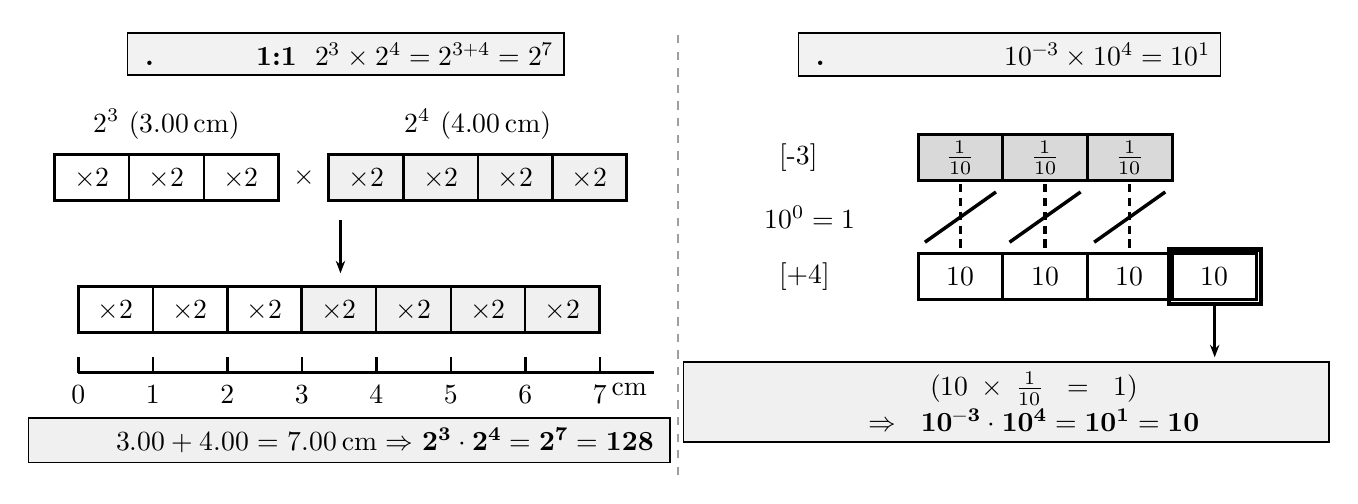
\begin{tikzpicture}[x=0.86cm, y=0.84cm, every node/.style={font=\linespread{1.0}\fontsize{10pt}{13pt}\selectfont, text=black}]
  \draw[line width=0.65pt, dashed, gray!75] (9.55, 0.05) -- (9.55, 6.80);
  \node[anchor=north, fill=headgray, draw=black, line width=0.6pt, inner sep=3.5pt] at (4.65, 6.75) {\textbf{ក. បន្ទះកត្តា \en{1:1}៖ $2^3\times 2^4 = 2^{3+4} = 2^7$}};
  \node[anchor=north, fill=headgray, draw=black, line width=0.6pt, inner sep=3.5pt] at (14.45, 6.75) {\textbf{ខ. ផ្ទាំងបន្សាបគូសូន្យ៖ $10^{-3}\times 10^4 = 10^1$}};

  % Left Panel: 1:1 Factor strips + ruler track
  \begin{scope}[shift={(0.35, 0.35)}]
    % 2^3 strip (3 units)
    \draw[black, line width=1.1pt, fill=white] (0, 3.85) rectangle (3.30, 4.55);
    \draw[black, line width=0.8pt] (1.10, 3.85) -- (1.10, 4.55) (2.20, 3.85) -- (2.20, 4.55);
    \node at (0.55, 4.20) {\en{$\times 2$}};
    \node at (1.65, 4.20) {\en{$\times 2$}};
    \node at (2.75, 4.20) {\en{$\times 2$}};
    \node[above=2pt] at (1.65, 4.55) {\en{$2^3$ ($3.00\unit{cm}$)}};
    % plus/times sign
    \node at (3.68, 4.20) {\textbf{\en{$\times$}}};
    % 2^4 strip (4 units)
    \draw[black, line width=1.1pt, fill=panelgray] (4.05, 3.85) rectangle (8.45, 4.55);
    \draw[black, line width=0.8pt] (5.15, 3.85) -- (5.15, 4.55) (6.25, 3.85) -- (6.25, 4.55) (7.35, 3.85) -- (7.35, 4.55);
    \node at (4.60, 4.20) {\en{$\times 2$}};
    \node at (5.70, 4.20) {\en{$\times 2$}};
    \node at (6.80, 4.20) {\en{$\times 2$}};
    \node at (7.90, 4.20) {\en{$\times 2$}};
    \node[above=2pt] at (6.25, 4.55) {\en{$2^4$ ($4.00\unit{cm}$)}};

    % Combined 7-unit strip on track
    \draw[black, line width=1.0pt, -{Stealth[length=4.5pt]}] (4.22, 3.55) -- (4.22, 2.75);
    \draw[black, line width=1.15pt, fill=white] (0.35, 1.85) rectangle (3.65, 2.55);
    \draw[black, line width=1.15pt, fill=panelgray] (3.65, 1.85) rectangle (8.05, 2.55);
    \foreach \x in {1.45, 2.55, 4.75, 5.85, 6.95} {
      \draw[black, line width=0.8pt] (\x, 1.85) -- (\x, 2.55);
    }
    \foreach \cx in {0.90, 2.00, 3.10, 4.20, 5.30, 6.40, 7.50} {
      \node at (\cx, 2.20) {\en{$\times 2$}};
    }
    % 0-8 cm track ruler below
    \draw[black, line width=1.0pt] (0.35, 1.25) -- (8.85, 1.25);
    \foreach \k/\lbl in {0/0, 1/1, 2/2, 3/3, 4/4, 5/5, 6/6, 7/7} {
      \draw[black, line width=0.85pt] (0.35+1.10*\k, 1.25) -- (0.35+1.10*\k, 1.48);
      \node[below=1pt] at (0.35+1.10*\k, 1.25) {\en{\lbl}};
    }
    \node[anchor=west] at (8.08, 1.00) {\en{cm}};
    \node[anchor=north, draw=black, fill=panelgray, line width=0.65pt, inner sep=3.5pt, text width=7.90cm, align=center] at (4.35, 0.58)
      {តប្រវែង៖ $3.00 + 4.00 = 7.00\unit{cm} \Rightarrow \mathbf{2^3\cdot 2^4 = 2^7 = 128}$};
  \end{scope}

  % Right Panel: 1:1 Signed Zero-Pair Cancellation Mat
  \begin{scope}[shift={(9.85, 0.35)}]
    % Negative 3 strip (hatched/shaded)
    \node[anchor=west] at (0.00, 4.50) {កត្តាចែក \en{[-3]}៖};
    \foreach \i in {0, 1, 2} {
      \fill[stepgray] (3.25+1.25*\i, 4.15) rectangle (4.50+1.25*\i, 4.85);
      \draw[black, line width=1.1pt] (3.25+1.25*\i, 4.15) rectangle (4.50+1.25*\i, 4.85);
      \node at (3.875+1.25*\i, 4.50) {\en{$\frac{1}{10}$}};
    }
    % Positive 4 strip
    \node[anchor=west] at (0.00, 2.70) {កត្តាគុណ \en{[+4]}៖};
    \foreach \i in {0, 1, 2, 3} {
      \fill[white] (3.25+1.25*\i, 2.35) rectangle (4.50+1.25*\i, 3.05);
      \draw[black, line width=1.1pt] (3.25+1.25*\i, 2.35) rectangle (4.50+1.25*\i, 3.05);
      \node at (3.875+1.25*\i, 2.70) {\en{$10$}};
    }
    % Zero-pair cancellation arrows / slashes
    \foreach \i in {0, 1, 2} {
      \draw[black, line width=1.15pt, densely dashed] (3.875+1.25*\i, 4.10) -- (3.875+1.25*\i, 3.10);
      \draw[black, line width=1.25pt] (3.35+1.25*\i, 3.22) -- (4.40+1.25*\i, 3.98);
    }
    \node[anchor=west, fill=white, inner sep=1pt] at (0.00, 3.60) {គូសូន្យ $10^0=1$};
    % Highlight surviving 4th cell
    \draw[black, line width=1.5pt] (6.95, 2.29) rectangle (8.31, 3.11);
    \draw[black, line width=1.0pt, -{Stealth[length=4.5pt]}] (7.63, 2.25) -- (7.63, 1.48);
    \node[anchor=north, draw=black, fill=panelgray, line width=0.65pt, inner sep=3.5pt, text width=7.95cm, align=center] at (4.55, 1.42)
      {កាត់ ៣ គូសូន្យ ($10\times\frac{1}{10}=1$) នៅសល់ ១ ប្រអប់ $\Rightarrow \mathbf{10^{-3}\cdot 10^4 = 10^1 = 10}$};
  \end{scope}
\end{tikzpicture}\par
\figcap{រូបទី ១៖}{គំនូសបច្ចេកទេស ស-ខ្មៅ នៃបន្ទះកត្តា \en{1:1} ($2^3\cdot 2^4 = 2^7$) និងផ្ទាំងបន្សាបគូសូន្យ ($10^{-3}\cdot 10^4 = 10^1$) ក្នុង \en{E2} សកម្មភាព ១ \en{(Guliman \& Alegre, 2021; Rini, 2022)}។}
\end{tcolorbox}

% --- រូបទី ២ ---
\Needspace{2.0cm}
\begin{tcolorbox}[enhanced, sharp corners, colback=white, colframe=black, boxrule=0.8pt, top=5pt, bottom=5pt, left=5pt, right=5pt, before skip=4pt, after skip=4pt]
\centering
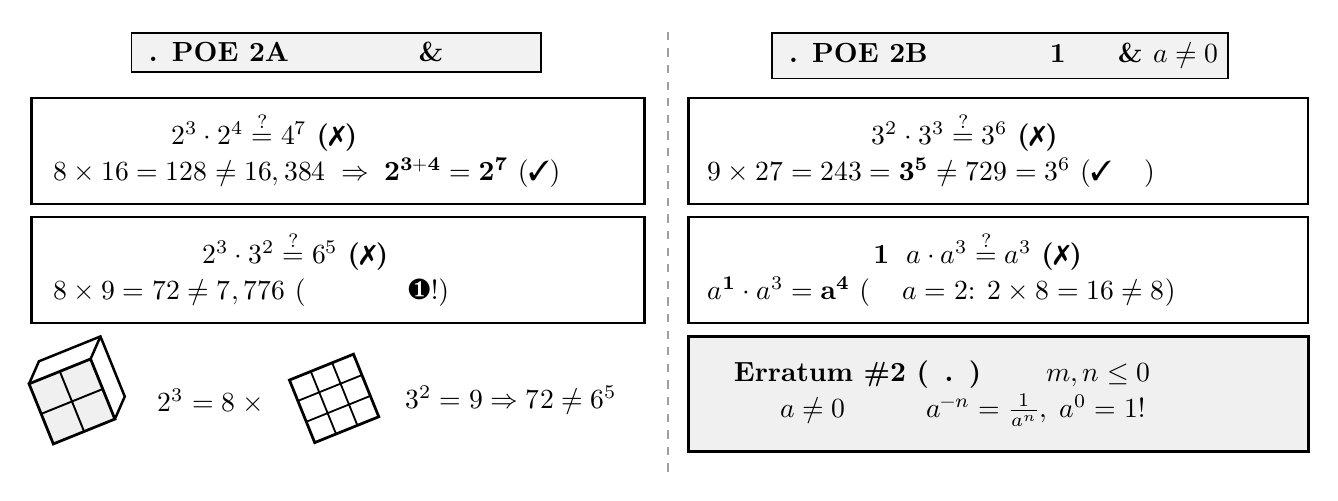
\begin{tikzpicture}[x=0.86cm, y=0.84cm, every node/.style={font=\linespread{1.0}\fontsize{10pt}{13pt}\selectfont, text=black}]
  \draw[line width=0.65pt, dashed, gray!75] (9.55, 0.05) -- (9.55, 6.75);
  \node[anchor=north, fill=headgray, draw=black, line width=0.6pt, inner sep=3.5pt] at (4.65, 6.70) {\textbf{ក. \en{POE 2A}៖ អន្ទាក់គុណគោល \& គោលខុសគ្នា}};
  \node[anchor=north, fill=headgray, draw=black, line width=0.6pt, inner sep=3.5pt] at (14.45, 6.70) {\textbf{ខ. \en{POE 2B}៖ គុណនិទស្សន្ត \en{1} លាក់ \& $a\neq 0$}};

  % Left Panel: POE 2A + rotated 22 deg B&W block grid
  \begin{scope}[shift={(0.15, 0.25)}]
    \draw[black, line width=0.9pt] (0, 3.85) rectangle (9.05, 5.45);
    \node[anchor=west, align=left] at (0.18, 4.65)
      {\textbf{ទាត់ចោលគុណគោល៖} $2^3\cdot 2^4 \stackrel{?}{=} 4^7$ \textbf{(\ding{55})}\\
       $8 \times 16 = 128 \neq 16,384 \;\Rightarrow\; \mathbf{2^{3+4} = 2^7}$ (\ding{51})};

    \draw[black, line width=0.9pt] (0, 2.05) rectangle (9.05, 3.65);
    \node[anchor=west, align=left] at (0.18, 2.85)
      {\textbf{ទាត់ចោលគោលខុសគ្នា៖} $2^3\cdot 3^2 \stackrel{?}{=} 6^5$ \textbf{(\ding{55})}\\
       $8 \times 9 = 72 \neq 7,776$ (បំពានច្រកគោល \cnum{1}!)};

    % Rotated 22 deg B&W grid visual (2x2x2 vs 3x3)
    \begin{scope}[shift={(0.32, 0.22)}, rotate=22]
      \draw[black, line width=1.0pt, fill=panelgray] (0,0) rectangle (0.98, 0.98);
      \draw[black, line width=0.7pt] (0.49,0)--(0.49,0.98) (0,0.49)--(0.98,0.49);
      \draw[black, line width=0.9pt] (0.98,0)--(1.24,0.26)--(1.24,1.24)--(0.26,1.24)--(0,0.98) (0.98,0.98)--(1.24,1.24);
    \end{scope}
    \node[anchor=west] at (1.72, 0.88) {\en{$2^3=8\;\times$}};
    \begin{scope}[shift={(4.18, 0.24)}, rotate=22]
      \draw[black, line width=1.0pt, fill=white] (0,0) rectangle (1.02, 1.02);
      \draw[black, line width=0.65pt] (0.34,0)--(0.34,1.02) (0.68,0)--(0.68,1.02) (0,0.34)--(1.02,0.34) (0,0.68)--(1.02,0.68);
    \end{scope}
    \node[anchor=west] at (5.38, 0.88) {\en{$3^2=9 \Rightarrow 72\neq 6^5$}};
  \end{scope}

  % Right Panel: POE 2B + Erratum #2 domain guard
  \begin{scope}[shift={(9.85, 0.25)}]
    \draw[black, line width=0.9pt] (0, 3.85) rectangle (9.15, 5.45);
    \node[anchor=west, align=left] at (0.14, 4.65)
      {\textbf{ទាត់ចោលគុណនិទស្សន្ត៖} $3^2\cdot 3^3 \stackrel{?}{=} 3^6$ \textbf{(\ding{55})}\\
       $9 \times 27 = 243 = \mathbf{3^5} \neq 729 = 3^6$ (\ding{51} បូក)};

    \draw[black, line width=0.9pt] (0, 2.05) rectangle (9.15, 3.65);
    \node[anchor=west, align=left] at (0.14, 2.85)
      {\textbf{អន្ទាក់និទស្សន្តលាក់ \en{1}៖} $a\cdot a^3 \stackrel{?}{=} a^3$ \textbf{(\ding{55})}\\
       $a^{\mathbf{1}}\cdot a^3 = \mathbf{a^4}$ (សាក $a=2$: $2\times 8 = 16 \neq 8$)};

    \draw[black, line width=1.1pt, fill=panelgray] (0, 0.10) rectangle (9.15, 1.85);
    \node[anchor=west, align=left] at (0.14, 0.98)
      {\textbf{កែ \en{Erratum \#2} (ទំ.១៥)៖} កាលណា $m, n \le 0$\\
       \textbf{ត្រូវមាន $a\neq 0$} និងស្ពាន $a^{-n}=\frac{1}{a^n},\; a^0=1$!};
  \end{scope}
\end{tikzpicture}\par
\figcap{រូបទី ២៖}{ពិសោធន៍ផ្ទុយ \en{Dual POE 2A--2B} រួមទាំងគំរូក្រឡាបង្វិល \en{22$^\circ$}, និទស្សន្តលាក់ \en{1} និងលក្ខខណ្ឌកំណត់ \en{Erratum \#2 ($a\neq 0$)} \en{(Maharani \& Subanji, 2018; Ulusoy, 2019; Şenay, 2024)}។}
\end{tcolorbox}

% --- រូបទី ៣ ---
\Needspace{2.0cm}
\begin{tcolorbox}[enhanced, sharp corners, colback=white, colframe=black, boxrule=0.8pt, top=5pt, bottom=5pt, left=5pt, right=5pt, before skip=4pt, after skip=4pt]
\centering
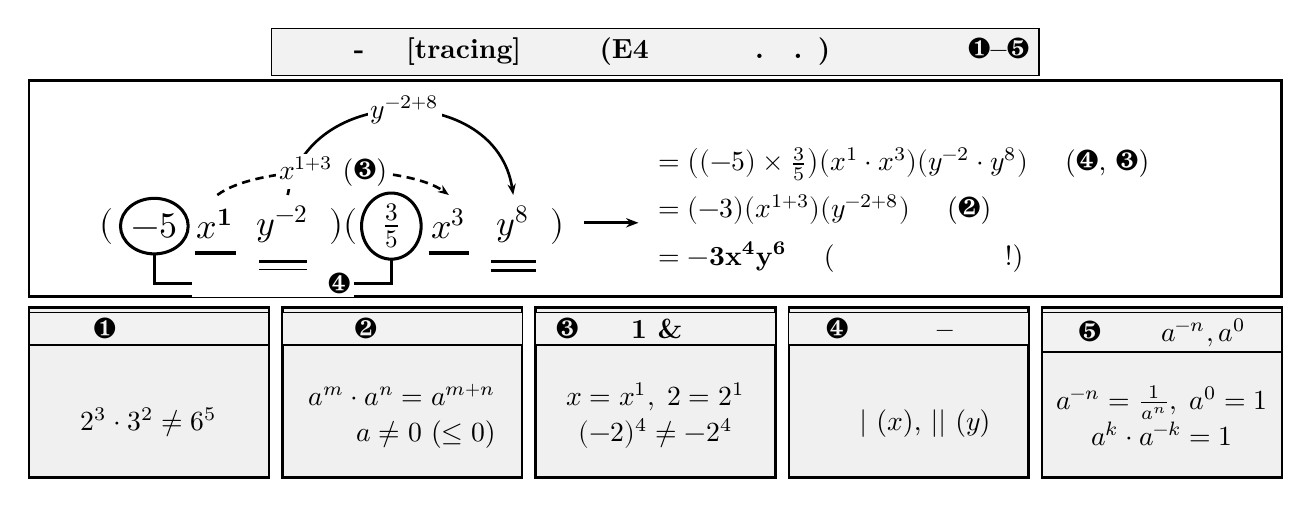
\begin{tikzpicture}[x=0.86cm, y=0.84cm, every node/.style={font=\linespread{1.0}\fontsize{10pt}{13pt}\selectfont, text=black}]
  \node[anchor=north, fill=headgray, draw=black, line width=0.6pt, inner sep=3.5pt] at (9.45, 6.95) {\textbf{កូដកម្ម ស-ខ្មៅ \en{[tracing]} ៣ ជំហាន (\en{E4} លំហាត់គំរូ គ. ទំ.១៥) និងធនាគារហេតុផល \cnum{1}--\cnum{5}}};

  % Top Tracing Blueprint box (extra headroom above arcs below y=6.15)
  \draw[black, line width=1.0pt, fill=white] (0.20, 2.88) rectangle (18.70, 6.15);
  % Monomial components positioned cleanly for tracing annotations
  \node at (1.35, 3.95) {\fontsize{13pt}{16pt}\selectfont\en{$($}};
  \node (c1) at (2.05, 3.95) {\fontsize{13pt}{16pt}\selectfont\en{$-5$}};
  \node (x1) at (2.95, 3.98) {\fontsize{13pt}{16pt}\selectfont\en{$x^{\mathbf{1}}$}};
  \node (y1) at (3.95, 3.98) {\fontsize{13pt}{16pt}\selectfont\en{$y^{-2}$}};
  \node at (4.85, 3.95) {\fontsize{13pt}{16pt}\selectfont\en{$)($}};
  \node (c2) at (5.55, 3.95) {\fontsize{13pt}{16pt}\selectfont\en{$\frac{3}{5}$}};
  \node (x2) at (6.40, 3.98) {\fontsize{13pt}{16pt}\selectfont\en{$x^{3}$}};
  \node (y2) at (7.35, 3.98) {\fontsize{13pt}{16pt}\selectfont\en{$y^{8}$}};
  \node at (8.00, 3.95) {\fontsize{13pt}{16pt}\selectfont\en{$)$}};

  % Circle coefficients
  \draw[black, line width=1.1pt] (2.05, 3.95) ellipse (0.50 and 0.42);
  \draw[black, line width=1.1pt] (5.55, 3.95) ellipse (0.44 and 0.50);
  % Single bar under x
  \draw[black, line width=1.25pt] (2.65, 3.54) -- (3.25, 3.54);
  \draw[black, line width=1.25pt] (6.10, 3.54) -- (6.70, 3.54);
  % Double bar under y
  \draw[black, line width=1.05pt] (3.60, 3.42) -- (4.30, 3.42) (3.60, 3.28) -- (4.30, 3.28);
  \draw[black, line width=1.05pt] (7.02, 3.42) -- (7.68, 3.42) (7.02, 3.28) -- (7.68, 3.28);
  % Overhead arcs connecting exponents (clean clearance from expression, each other, and y=6.15 top border)
  \draw[black, line width=0.95pt, -{Stealth[length=4pt]}] (4.02, 4.42) .. controls (4.30, 6.12) and (7.10, 6.12) .. (7.35, 4.42);
  \node[fill=white, inner sep=1pt] at (5.75, 5.70) {\en{$y^{-2+8}$}};
  \draw[black, line width=0.95pt, densely dashed, -{Stealth[length=4pt]}] (2.98, 4.42) .. controls (3.60, 4.90) and (5.75, 4.90) .. (6.40, 4.42);
  \node[fill=white, inner sep=1pt] at (4.69, 4.78) {\en{$x^{1+3}$ (\cnum{3})}};
  % Bottom connector for coefficients
  \draw[black, line width=0.95pt] (2.05, 3.52) -- (2.05, 3.08) -- (5.55, 3.08) -- (5.55, 3.45);
  \node[fill=white, inner sep=1pt] at (3.80, 3.08) {ព័ទ្ធរង្វង់មេគុណ \cnum{4}};

  % Step-by-step right side of top box
  \draw[black, line width=1.1pt, -{Stealth[length=4.5pt]}] (8.40, 4.00) -- (9.20, 4.00);
  \node[anchor=west, align=left] at (9.35, 4.20)
    {$= \bigl((-5)\times \frac{3}{5}\bigr)(x^1\cdot x^3)(y^{-2}\cdot y^8)$ \quad (\cnum{4}, \cnum{3})\\[4pt]
     $= (-3)(x^{1+3})(y^{-2+8})$ \quad (\cnum{2})\\[4pt]
     $= \mathbf{-3x^4y^6}$ \quad (ការពារសញ្ញាដកមុខឯកធាតុ!)};

  % Bottom 5 Warrant Bank cards
  \draw[black, line width=0.9pt, fill=panelgray] (0.20, 0.15) rectangle (3.74, 2.72);
  \node[anchor=north, fill=headgray, draw=black, line width=0.5pt, inner sep=2pt, minimum width=3.05cm] at (1.97, 2.65) {\textbf{\cnum{1} ច្រកគោលដូច}};
  \node[anchor=center, align=center] at (1.97, 1.08) {គោលដូចគ្នាទើបបូក\\ $2^3\cdot 3^2\neq 6^5$};

  \draw[black, line width=0.9pt, fill=panelgray] (3.94, 0.15) rectangle (7.48, 2.72);
  \node[anchor=north, fill=headgray, draw=black, line width=0.5pt, inner sep=2pt, minimum width=3.05cm] at (5.71, 2.65) {\textbf{\cnum{2} វិធានគុណ}};
  \node[anchor=center, align=center] at (5.71, 1.08) {$a^m\cdot a^n=a^{m+n}$\\ ត្រូវ $a\neq 0$ ($\le 0$)};

  \draw[black, line width=0.9pt, fill=panelgray] (7.68, 0.15) rectangle (11.22, 2.72);
  \node[anchor=north, fill=headgray, draw=black, line width=0.5pt, inner sep=2pt, minimum width=3.05cm] at (9.45, 2.65) {\textbf{\cnum{3} លាក់ \en{1} \& វង់ក្រចក}};
  \node[anchor=center, align=center] at (9.45, 1.08) {$x=x^1,\; 2=2^1$\\ $(-2)^4\neq -2^4$};

  \draw[black, line width=0.9pt, fill=panelgray] (11.42, 0.15) rectangle (14.96, 2.72);
  \node[anchor=north, fill=headgray, draw=black, line width=0.5pt, inner sep=2pt, minimum width=3.05cm] at (13.19, 2.65) {\textbf{\cnum{4} ផ្ដុំមេគុណ--អក្សរ}};
  \node[anchor=center, align=center] at (13.19, 1.08) {ព័ទ្ធមេគុណជាប់ដក\\ គូស \en{|} ($x$), \en{||} ($y$)};

  \draw[black, line width=0.9pt, fill=panelgray] (15.16, 0.15) rectangle (18.70, 2.72);
  \node[anchor=north, fill=headgray, draw=black, line width=0.5pt, inner sep=2pt, minimum width=3.05cm] at (16.93, 2.65) {\textbf{\cnum{5} ស្ពាន $a^{-n}, a^0$}};
  \node[anchor=center, align=center] at (16.93, 1.08) {$a^{-n}=\frac{1}{a^n},\; a^0=1$\\ $a^k\cdot a^{-k}=1$};
\end{tikzpicture}\par
\figcap{រូបទី ៣៖}{គំរូកូដកម្ម ស-ខ្មៅ \en{[tracing]} លើលំហាត់គំរូ គ. ទំ.១៥ និងធនាគារហេតុផល \cnum{1}--\cnum{5} (ទំព័រ ២ និង ៤) \en{(Yeo \& Tzeng, 2019; Aydın-Güç \& Aygün, 2021; Wang et al., 2026)}។}
\end{tcolorbox}

% --- រូបទី ៤ ---
\Needspace{2.0cm}
\begin{tcolorbox}[enhanced, sharp corners, colback=white, colframe=black, boxrule=0.8pt, top=3pt, bottom=3pt, left=5pt, right=5pt, before skip=2pt, after skip=2pt]
\centering
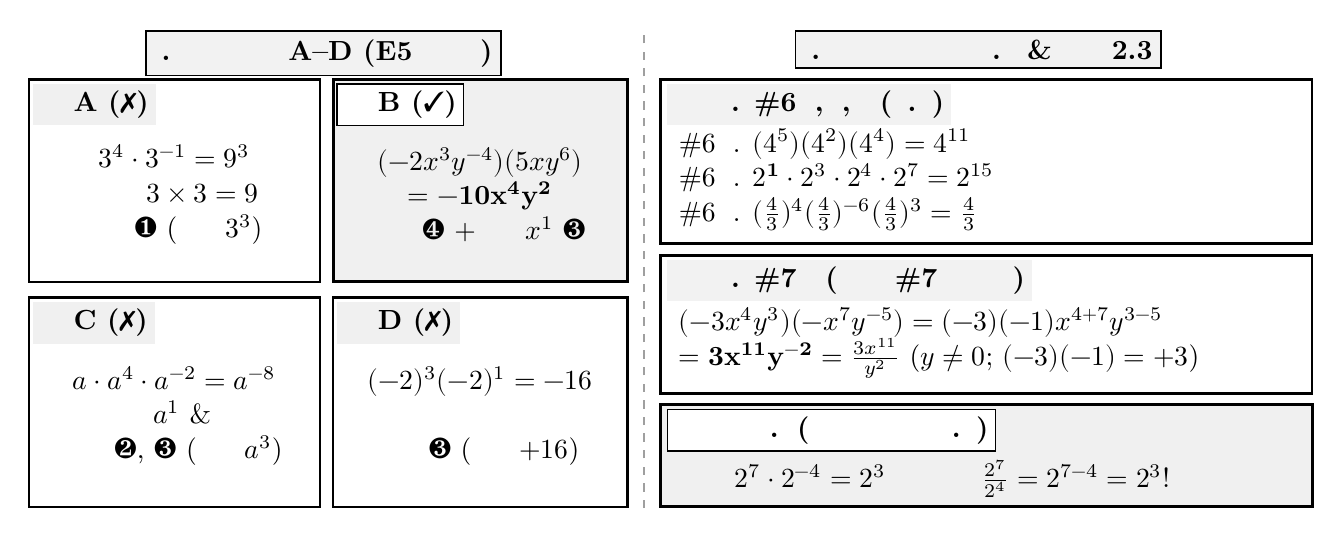
\begin{tikzpicture}[x=0.84cm, y=0.81cm, every node/.style={font=\linespread{1.0}\fontsize{10pt}{12.5pt}\selectfont, text=black}]
  \draw[line width=0.65pt, dashed, gray!75] (9.40, 0.00) -- (9.40, 7.52);
  \node[anchor=north, fill=headgray, draw=black, line width=0.6pt, inner sep=3pt] at (4.55, 7.49) {\textbf{ក. កាតវិនិច្ឆ័យ \en{A--D} \en{(E5} ទំព័រ ៥\en{)}}};
  \node[anchor=north, fill=headgray, draw=black, line width=0.6pt, inner sep=3pt] at (14.45, 7.49) {\textbf{ខ. ផែនទីកិច្ចការផ្ទះ ទំ.២៥ \en{\&} ស្ពាន \en{2.3}}};

  % Left 2x2 Diagnostic Foils A-D
  \draw[black, line width=0.9pt] (0.10, 3.55) rectangle (4.50, 6.72);
  \node[anchor=north west, fill=panelgray, inner sep=2.5pt] at (0.15, 6.66) {\textbf{កាត \en{A (\ding{55})}}};
  \node[align=center] at (2.30, 4.92) {$3^4\cdot 3^{-1} = 9^3$\\ គុណគោល $3\times 3=9$\\ បំពាន \cnum{1} (ត្រូវ $3^3$)};

  \draw[black, line width=1.2pt, fill=panelgray] (4.70, 3.55) rectangle (9.15, 6.72);
  \node[anchor=north west, fill=white, draw=black, line width=0.5pt, inner sep=2.5pt] at (4.75, 6.66) {\textbf{កាត \en{B (\ding{51})}}};
  \node[align=center] at (6.92, 4.92) {$(-2x^3y^{-4})(5xy^6)$\\ $= \mathbf{-10x^4y^2}$\\ ផ្ដុំ \cnum{4} + លាក់ $x^1$ \cnum{3}};

  \draw[black, line width=0.9pt] (0.10, 0.02) rectangle (4.50, 3.30);
  \node[anchor=north west, fill=panelgray, inner sep=2.5pt] at (0.15, 3.24) {\textbf{កាត \en{C (\ding{55})}}};
  \node[align=center] at (2.30, 1.45) {$a\cdot a^4\cdot a^{-2} = a^{-8}$\\ ភ្លេច $a^1$ \& គុណ\\ បំពាន \cnum{2}, \cnum{3} (ត្រូវ $a^3$)};

  \draw[black, line width=0.9pt] (4.70, 0.02) rectangle (9.15, 3.30);
  \node[anchor=north west, fill=panelgray, inner sep=2.5pt] at (4.75, 3.24) {\textbf{កាត \en{D (\ding{55})}}};
  \node[align=center] at (6.92, 1.45) {$(-2)^3(-2)^1 = -16$\\ ដែនវង់ក្រចកគូ\\ បំពាន \cnum{3} (ត្រូវ $+16$)};

  % Right 3 HW & Bridge boxes (extra vertical headroom so fractions never touch borders)
  \draw[black, line width=0.9pt] (9.65, 4.15) rectangle (19.50, 6.72);
  \node[anchor=north west, fill=headgray, inner sep=2.5pt] at (9.74, 6.66) {\textbf{ផ្នែក ក. \en{\#6} ក, ខ, គ (ទំ.២៥)}};
  \node[anchor=north west, align=left] at (9.78, 6.10)
    {\en{\#6} ក. $(4^5)(4^2)(4^4)=4^{11}$\\
     \en{\#6} ខ. $2^{\mathbf{1}}\cdot 2^3\cdot 2^4\cdot 2^7=2^{15}$\\
     \en{\#6} គ. $(\frac{4}{3})^4(\frac{4}{3})^{-6}(\frac{4}{3})^3=\frac{4}{3}$};

  \draw[black, line width=0.9pt] (9.65, 1.80) rectangle (19.50, 3.96);
  \node[anchor=north west, fill=headgray, inner sep=2.5pt] at (9.74, 3.90) {\textbf{ផ្នែក ខ. \en{\#7} ខ (ជៀសវាង \en{\#7} ក ខ្វះតួ)}};
  \node[anchor=north west, align=left] at (9.78, 3.30)
    {$(-3x^4y^3)(-x^7y^{-5}) = (-3)(-1)x^{4+7}y^{3-5}$\\
     $= \mathbf{3x^{11}y^{-2}} = \frac{3x^{11}}{y^2}$ ($y\neq 0$; $(-3)(-1)=+3$)};

  \draw[black, line width=1.1pt, fill=panelgray] (9.65, 0.02) rectangle (19.50, 1.62);
  \node[anchor=north west, fill=white, draw=black, line width=0.5pt, inner sep=2.5pt] at (9.74, 1.56) {\textbf{ស្ពានមេរៀន ២.៣ (វិធីចែកស្វ័យគុណ ទំ.១៦)}};
  \node[anchor=north west, align=left] at (9.78, 0.90)
    {ផ្ទៀង៖ $2^7\cdot 2^{-4} = 2^3$ \;\;ធៀបនឹង\;\; $\frac{2^7}{2^4} = 2^{7-4} = 2^3$!};
\end{tikzpicture}\par
\figcap{រូបទី ៤៖}{កាតវិនិច្ឆ័យ \en{A--D} (ទំព័រ ៥) និងផែនទីកិច្ចការផ្ទះទំ.២៥ (\en{\#6} ក, ខ, គ, \en{\#7} ខ) ភ្ជាប់ស្ពានមេរៀន \en{2.3} \en{(Pournara \& Bowie, 2023; Olson et al., 2011; Aydın-Güç \& Aygün, 2021)}។}
\end{tcolorbox}

% ============================================================================
% ផ្នែកទី ៦៖ តារាងភស្តុតាង ១៥ ឯកសារ ការក្រិតបោះពុម្ព & ចម្លើយគំរូពេញលេញ
% ============================================================================
\secbanner{ផ្នែកទី ៦៖ តារាងភស្តុតាង \enbf{15 PDFs,} ការក្រិតបោះពុម្ព \enbf{\&} ចម្លើយគំរូ \enbf{(Pages 1--6)}}{Section 6: Complete Evidence Alignment Table (01--15), Printing Calibration (1:1) \& Master Answer Keys}

\subsec{៦\enbf{.}១ តារាងភស្តុតាងស្រាវជ្រាវ \enbf{Open-Access (01--15)} ផ្ទៀងផ្ទាត់ \enbf{1-to-1}}

តារាងខាងក្រោមផ្គូផ្គងឯកសារ \en{PDF} ទាំង \en{15} ច្បាប់ក្នុងថត ឯកសារស្រាវជ្រាវយោង\en{\_PDF} តាមលំដាប់អក្ខរក្រម \en{APA 7th (01--15)} ជាមួយលទ្ធផលពិសោធន៍ពិត និងចំណុចអនុវត្តក្នុងមេរៀន \en{2.2}៖

\begingroup
\linespread{1.0}\fontsize{10.2pt}{15.5pt}\selectfont
\renewcommand{\arraystretch}{1.28}
\begin{longtable}{|C{1.10cm}|L{3.45cm}|L{6.25cm}|L{6.05cm}|}
\hline
\rowcolor{headgray}
\multicolumn{1}{|C{1.10cm}|}{\tblhead{\enbf{\#}}} &
\multicolumn{1}{C{3.45cm}|}{\tblhead{ប្រភព \enbf{APA 7th}}} &
\multicolumn{1}{C{6.25cm}|}{\tblhead{លទ្ធផលពិសោធន៍ស្នូល}} &
\multicolumn{1}{C{6.05cm}|}{\tblhead{ការរួមបញ្ចូលក្នុងមេរៀន \enbf{2.2} \& សន្លឹកកិច្ចការ}} \\
\hline
\endfirsthead
\hline
\rowcolor{headgray}
\multicolumn{1}{|C{1.10cm}|}{\tblhead{\enbf{\#}}} &
\multicolumn{1}{C{3.45cm}|}{\tblhead{ប្រភព \enbf{APA 7th}}} &
\multicolumn{1}{C{6.25cm}|}{\tblhead{លទ្ធផលពិសោធន៍ស្នូល}} &
\multicolumn{1}{C{6.05cm}|}{\tblhead{ការរួមបញ្ចូលក្នុងមេរៀន \enbf{2.2} \& សន្លឹកកិច្ចការ}} \\
\hline
\endhead
\hline
\endfoot
\hline
\endlastfoot
\textbf{\en{01}} & \en{\textbf{Aydın-Güç \& Aygün (2021)}} \newline (\en{21 pp.}) & ថ្នាក់ទី៨ \en{N = 48 (pp. 1116--1118)}៖ \en{50\% (n = 24)} ភ្លេចសញ្ញាដកមុខឯកធាតុ (\en{«No need to pay attention»}); \en{25\%} ពន្លាតខុស។ & ការពារសញ្ញាដកមុខ $(-5xy^{-2})(\frac{3}{5}x^3y^8)$, ប្រតិបត្តិ គ. (\en{Erratum \#1}), និង \en{\#7} ខ. $(-3x^4y^3)(-x^7y^{-5})$។ \\
\hline
\textbf{\en{02}} & \en{\textbf{Barbieri \& Booth (2016)}} \newline (\en{32 pp.}) & \en{RCT} ទី៨ \en{N = 125}៖ ឧទាហរណ៍ខុស + សញ្ញាកំហុស (\en{$\beta$ = -.182, p = .045}) ជួយសិស្សខ្សោយ (\en{p = .793 vs .003}) និងរក្សាចំណាប់អារម្មណ៍ (\en{p = .025})។ & កែ \en{Erratum \#1} និងសួរវិនិច្ឆ័យកំហុស \en{EIA / Pause-Review} លើ \en{E4--E5} (ទំព័រ ២, ៣, ៥)។ \\
\hline
\textbf{\en{03}} & \en{\textbf{Guliman \& Alegre (2021)}} \newline (\en{7 pp.}) & ថ្នាក់ទី៨ \en{N = 70}៖ បន្ទះកាក់ស្វ័យគុណបង្កើនពិន្ទុពី \en{39.73\% $\to$ 81.20\% (p = .007)}, ប្រយោជន៍ \en{4.44/5.00}។ & រចនាបន្ទះកត្តា ស-ខ្មៅ \en{1:1} ($2^3: 3.00\unit{cm}$ និង $2^4: 4.00\unit{cm}$) លើទំព័រ ១ (\en{E2} ស.១)។ \\
\hline
\textbf{\en{04}} & \en{\textbf{Gustina et al. (2023)}} \newline (\en{13 pp.}) & មេតាវិភាគ \en{70} សំណុំទិន្នន័យ (\en{17 JHS})៖ \en{POE} ឈានដល់ \en{RE = 0.67 [0.40, 0.94]} ក្នុងគណិតវិទ្យា (រួម \en{0.60, p < .001})។ & ប្រើវដ្ដទស្សន៍ទាយ--សង្កេត--ពន្យល់ក្នុង \en{E1} ម៉ាស៊ីនមេ និង \en{Dual POE 2A--2B} (ទំព័រ ១)។ \\
\hline
\textbf{\en{05}} & \en{\textbf{Maharani \& Subanji (2018)}} \newline (\en{8 pp.}) & ថ្នាក់ទី៨ \en{N = 25 (45.4\%} កំហុសតំណាង\en{)}៖ ជម្លោះគំនិត + ឧទាហរណ៍ផ្ទុយ + \en{Scaffolding} កម្រិត $\gamma$។ & បង្កើត \en{Dual POE 2A--2B} ($2^3\cdot 2^4\neq 4^7,\; 2^3\cdot 3^2\neq 6^5,\; 3^2\cdot 3^3\neq 3^6,\; a\cdot a^3\neq a^3$)។ \\
\hline
\textbf{\en{06}} & \en{\textbf{Olson et al. (2011)}} \newline (\en{8 pp.}) & \en{N = 904; n = 19} សម្ភាសន៍៖ មានតែ \en{5/19} ញែក $(-17)^8$ \en{vs} $-17^8$; ទាក់ទងការយល់ $n^{-1}$។ & គាំទ្រហេតុផល \cnum{3} (ដែនវង់ក្រចក), កែកិច្ចការផ្ទះ $(-2)^7, (-8)^6$ និងកាត \en{D} $(-2)^4=-16$។ \\
\hline
\textbf{\en{07}} & \en{\textbf{Pournara \& Bowie (2023)}} \newline (\en{11 pp.}) & \en{N = 589} (\en{473} ទី៧ + \en{116} ទី៨)៖ លើ $3^2+3^3$ ត្រឹម \en{28.2\%} ត្រូវ, \en{54.5\%--60\%} ច្រឡំស្វ័យគុណ ($6^5$ \en{36.2\%})។ & រចនា \en{Diagnostic Exit Foils A--D} ចម្រុះទម្រង់ និងសំបុត្រចេញ \en{Q3} ($2^3\cdot 3^2\neq 6^5$, ទំព័រ ៥)។ \\
\hline
\textbf{\en{08}} & \en{\textbf{Pournara et al. (2016)}} \newline (\en{10 pp.}) & \en{N = 250}៖ បូក $2a+5a\to 7a^2$ (\en{10\%--17\%}), $2a+5b\to 7ab$ (\en{42\%--53\%}), មើលលេខមុនអក្សរ (\en{47\%--59\%})។ & ផ្ដុំមេគុណនិងអញ្ញាតដាច់ដោយឡែកតាម \cnum{4} ក្នុង \en{E4} (ទំព័រ ២) និងព្រមានមិនប្រើច្បាប់លើផលបូក។ \\
\hline
\textbf{\en{09}} & \en{\textbf{Rini (2022)}} \newline (\en{14 pp.}) & ថ្នាក់ទី៧ \en{n = 36}៖ ដំណាក់កាល ៣ ជំហាន រូបី $\to$ លុបគូសូន្យ (\en{zero-pair}) $\to$ និមិត្តសញ្ញា។ & គាំទ្រផ្ទាំងលុបគូសូន្យ $10^{-3}\times 10^4=10^1$ ($10\times\frac{1}{10}=10^0=1$) មុនផ្ទេរទៅ \en{E4}។ \\
\hline
\textbf{\en{10}} & \en{\textbf{Şenay (2024)}} \newline (\en{15 pp.}) & ទិន្នន័យ ៥ (\en{N = 729; N = 159} ទី៨)៖ \en{34\%} ជំនួសទ្រឹស្ដីដោយគណនា, លុបវង់ក្រចក, រំលងប្រភាគ $<1$។ & ការពារគោលប្រភាគ $(\frac{3}{2})^2(\frac{3}{2})^3$, $(-\frac{3}{2})^2(-\frac{3}{2})^{-2}$ និងលក្ខខណ្ឌ \en{Erratum \#2 ($a\neq 0$)}។ \\
\hline
\textbf{\en{11}} & \en{\textbf{Turan \& Matteson (2021)}} \newline (\en{19 pp.}) & គ្រូ ៧ នាក់ (\en{14} មេរៀន)៖ \en{E3} ធ្លាក់ដល់ \en{1.6}, \textbf{\en{E4 = 0} គ្រប់មេរៀន}, \en{E5} រុញទៅផ្ទះ។ & ចាក់សោពេល \en{2+9+17+20+$\le$2} ឱ្យសិស្សបង្គុំ \en{E3} មុនគ្រូ និងបញ្ចប់ \en{E4--E5} ក្នុងថ្នាក់។ \\
\hline
\textbf{\en{12}} & \en{\textbf{Ulusoy (2019)}} \newline (\en{19 pp.}) & ទី៨ \en{N = 165}៖ តែ \en{3.5\%} ត្រូវគ្រប់សំណួរ; ខុសលើ $-3^0$ (\en{66.1\%}), $2^{-4}$ (\en{63.6\%}), $5^{-2}\cdot 5^4$ (\en{59.4\%}), $5^{-4}\cdot 6^4$ (\en{61.8\%})។ & ជាគ្រឹះស្នូលនៃ \en{POE 2A--2B}, ធនាគារ \cnum{1}--\cnum{5}, កាត \en{A--D} និងសំបុត្រចេញ ($5^{-2}\cdot 5^6$)។ \\
\hline
\textbf{\en{13}} & \en{\textbf{Wang et al. (2026)}} \newline (\en{11 pp.}) & \en{N = 134}៖ ក្រុម ៣ នាក់បន្ថយបន្ទុកគិត (\en{p < .01}) និងពូកែផ្ទេរស្មុគស្មាញតែពេលមានគ្រឹះរឹងមាំ (\en{p < .05})។ & បង្រៀនគ្រឹះ \en{E2/E3} ឱ្យមាំមុនផ្ទេរទៅ \en{Relay} ៣ តួនាទី \en{E5} (ទំព័រ ៣)។ \\
\hline
\textbf{\en{14}} & \en{\textbf{Wesenberg et al. (2022)}} \newline (\en{20 pp.}) & \en{N = 83}៖ ដាក់ឧទាហរណ៍ត្រូវមុនខុស (\en{CE--EE}) បន្ថយបន្ទុកគិត (\en{p = .037}) និងជួយការផ្ទេរពន្យារ។ & រៀបលំដាប់ច្បាប់ត្រូវ \en{E2--E4} មុនកាតខុស \en{A, C, D} និងកែ \en{Erratum \#1} នៅ \en{E5}។ \\
\hline
\textbf{\en{15}} & \en{\textbf{Yeo \& Tzeng (2019)}} \newline (\en{11 pp.}) & \en{N = 72}៖ \en{[tracing]} បង្កើនពិន្ទុផ្ទេរ (\en{p = .003, $\eta^2$ = .121}) និងបន្ថយលំបាកគិត (\en{p < .001}) គ្រប់ \en{WMC}។ & ដាក់សញ្ញា ស-ខ្មៅ \en{[tracing]} ព័ទ្ធមេគុណ គូស \en{|} ($x$), \en{||} ($y$), ធ្នូនិទស្សន្តលើ \en{E4} (ទំ.២)។ \\
\hline
\end{longtable}
\endgroup

\subsec{៦\enbf{.}២ ស្តង់ដារបោះពុម្ព \enbf{Actual Size 100\%} និងលំដាប់ចែកសន្លឹកកិច្ចការ \enbf{(Pages 1--6)}}

\begin{enumerate}[leftmargin=0.65cm, itemsep=2.2pt]
  \item \textbf{ការកំណត់បោះពុម្ព \en{1:1} ដាច់ខាត (ទំព័រ ១)៖} បោះពុម្ពឯកសារ \en{Printable\_Materials\_EXP\_MUL.pdf} ដោយជ្រើស \textbf{\en{Scale: Actual Size 100\%}} (\textit{ហាមប្រើ} \en{Fit to Page / Shrink to Fit}) ហើយវាស់ផ្ទៀង\textbf{បន្ទះក្រិត \en{5.00 cm}} (\en{141.73 pt}) នៅខាងស្ដាំផ្នែកខាងលើទំព័រ ១ ដើម្បីធានាថា បន្ទះកត្តា $2^3$ ($3.00\unit{cm}$), $2^4$ ($4.00\unit{cm}$), បន្ទាត់ $0\text{--}8\unit{cm}$, និងផ្ទាំងបន្សាបគូសូន្យ $10^{-3}\times 10^4$ មានខ្នាត \en{1:1} ពិតប្រាកដ។
  \item \textbf{ការបែងចែកសន្លឹក ស-ខ្មៅ សន្សំក្រដាស (ទំព័រ ២--៦)៖} ទំព័រ ២ (កាត \en{E4} គំរូ ក, ខ, គ) និងទំព័រ ៣ (សន្លឹក \en{E5} ប្រតិបត្តិ ៣ តួនាទី) ជាទម្រង់បត់/កាត់ \en{2-up}; ទំព័រ ៤ (ផ្ទាំងធនាគារហេតុផល \cnum{1}--\cnum{5} និងដែនវង់ក្រចក) គួរព្រីនលើក្រដាសរឹង \en{180 gsm} បិទលើក្ដារខៀន; ទំព័រ ៥ ជាកាត \en{A--D} + ចម្លើយគ្រូ + សំបុត្រចេញ ៣ សំណួរ; និងទំព័រ ៦ ជាប័ណ្ណកិច្ចការផ្ទះកាត់ចែក។
  \item \textbf{ឧបករណ៍តុក្រុម ៣ នាក់ និងនាទីចែកសន្លឹក៖} កន្ត្រៃ ១, បន្ទាត់ក្រិត \en{cm} ១, និងខ្មៅដៃ \en{[tracing]} ក្នុងមួយក្រុម។ ចែកទំព័រ ១ ផ្កាប់នៅនាទី ០០', ទំព័រ ២ នៅនាទី ២៨', ទំព័រ ៣ នៅនាទី ៣៨', ទំព័រ ៥ នៅនាទី ៤៣', និងទំព័រ ៦ នៅនាទី ៤៨'។
\end{enumerate}

\subsec{៦\enbf{.}៣ ចម្លើយគំរូពេញលេញសម្រាប់គ្រប់សន្លឹកកិច្ចការ \enbf{(Pages 1--6 \& HW)}}

\begingroup
\linespread{1.06}\fontsize{10.2pt}{15.8pt}\selectfont
\renewcommand{\arraystretch}{1.38}
\begin{longtable}{|L{3.00cm}|L{14.15cm}|}
\hline
\rowcolor{headgray}
\multicolumn{1}{|C{3.00cm}|}{\tblhead{សន្លឹក \enbf{/} លំហាត់}} &
\multicolumn{1}{C{14.15cm}|}{\tblhead{ចម្លើយគំរូផ្លូវការ និងពិន្ទុត្រួតពិនិត្យ \enbf{(Master Key)}}} \\
\hline
\endfirsthead
\hline
\rowcolor{headgray}
\multicolumn{1}{|C{3.00cm}|}{\tblhead{សន្លឹក \enbf{/} លំហាត់}} &
\multicolumn{1}{C{14.15cm}|}{\tblhead{ចម្លើយគំរូផ្លូវការ និងពិន្ទុត្រួតពិនិត្យ \enbf{(Master Key)}}} \\
\hline
\endhead
\hline
\endfoot
\hline
\endlastfoot
\textbf{ទំព័រ ១ (\en{E2})} \newline បន្ទះ \en{1:1} \newline ($2^3\cdot 2^4$ \& $10^{-3}\cdot 10^4$) &
\textbf{សកម្មភាព ១៖} តបន្ទះ $2^3$ ($3.00\unit{cm}$) និង $2^4$ ($4.00\unit{cm}$) លើបន្ទាត់ $0\text{--}8\unit{cm} \Rightarrow 7.00\unit{cm} \Rightarrow \mathbf{2^3\cdot 2^4 = 2^{3+4} = 2^7 = 128}$។ \newline
លើផ្ទាំងគូសូន្យ $10^{-3}\times 10^4$៖ កាត់ ៣ គូនៃ $10\times \frac{1}{10} = 10^0 = 1$ នៅសល់ ១ ប្រអប់ $10 \Rightarrow \mathbf{10^{-3+4} = 10^1 = 10}$។ \\
\hline
\textbf{ទំព័រ ១ (\en{E2})} \newline \en{Dual POE 2A--2B} &
\textbf{\en{POE 2A}៖} $2^3\cdot 2^4 = 8\times 16 = 128 \neq 16,384 = 4^7$ (\textbf{ខុស} — រក្សាគោល $2^7$); $2^3\cdot 3^2 = 8\times 9 = 72 \neq 7,776 = 6^5$ (\textbf{ខុស} — គោលខុសគ្នាបូកនិទស្សន្តមិនបាន \cnum{1})។ \newline
\textbf{\en{POE 2B}៖} $3^2\cdot 3^3 = 9\times 27 = 243 = \mathbf{3^5} \neq 729 = 3^6$ (\textbf{ខុស} — ត្រូវបូក); $a\cdot a^3 = a^{\mathbf{1}}\cdot a^3 = \mathbf{a^4} \neq a^3$ (សាក $a=2 \Rightarrow 16\neq 8$)។ \\
\hline
\textbf{ទំព័រ ២ (\en{E4})} \newline លំហាត់គំរូ \newline (ទំ.១៥ ក, ខ, គ) &
\textbf{ក.} $10^{-3}\times 10^4 = 10^{-3+4} = 10^1 = \mathbf{10}$ (\cnum{2})។ \newline
\textbf{ខ.} $(-5y^2)(7y^8) = (-5\times 7)(y^2\cdot y^8) = -35y^{2+8} = \mathbf{-35y^{10}}$ (\cnum{4}, \cnum{2})។ \newline
\textbf{គ.} $(-5xy^{-2})(\frac{3}{5}x^3y^8) = (-5\times\frac{3}{5})(x^{\mathbf{1}}\cdot x^3)(y^{-2}\cdot y^8) = \mathbf{-3x^4y^6}$ ($y\neq 0$; ប្រយ័ត្នសញ្ញាដកមុខ $-3$ និង $x^1$)។ \newline
\textbf{\en{EIA 30s}៖} ១) សញ្ញាដក $(-5)\times\frac{3}{5}=-3$ រក្សាទុក; ២) បើភ្លេច $x=x^1$ នឹងខុសជា $x^3$។ \\
\hline
\textbf{ទំព័រ ៣ (\en{E5})} \newline ប្រតិបត្តិ ៣ តួនាទី \newline (ទំ.១៥ ក, ខ, គ) &
\textbf{ក.} $x^9\cdot x^4 = x^{9+4} = \mathbf{x^{13}}$ (\cnum{2})។ \quad
\textbf{ខ.} $(-\frac{3}{2})^2\cdot(-\frac{3}{2})^{-2} = (-\frac{3}{2})^{2+(-2)} = (-\frac{3}{2})^0 = \mathbf{1}$ (\cnum{2}, \cnum{5})។ \newline
\textbf{គ. (កែ \en{Erratum \#1}):} $(3x^4y^{-3})(-\frac{4}{3}x^{-2}y) = (3\times -\frac{4}{3})(x^4\cdot x^{-2})(y^{-3}\cdot y^{\mathbf{1}}) = \mathbf{-4x^2y^{-2}}$ ($= -\frac{4x^2}{y^2},\; x,y\neq 0$)។ \newline
\textbf{បិទ \en{E1} ម៉ាស៊ីនមេ៖} វីដេអូសរុប $= 2^3\cdot 2^4 = 2^7 = \mathbf{128}$ វីដេអូ; ទិន្នន័យ $= 10^{-3}\cdot 10^4 = \mathbf{10\unit{MB}}$។ \\
\hline
\textbf{ទំព័រ ៤ (\en{Poster})} \newline ធនាគារ \cnum{1}--\cnum{5} &
\cnum{1} ច្រកគោលដូចគ្នា ($a^m\cdot b^n$ បូកនិទស្សន្តមិនបាន) \;\vert\; \cnum{2} $a^m\cdot a^n = a^{m+n}$ (\textbf{ត្រូវ $a\neq 0$} កាលណា $m,n\le 0$) \;\vert\; \cnum{3} និទស្សន្តលាក់ $1$ ($x^1, y^1, 2^1$) \& ដែនវង់ក្រចក ($-2^4=-16 \neq (-2)^4=+16$) \;\vert\; \cnum{4} ផ្ដុំមេគុណជាប់សញ្ញាដក \& គូស \en{|}, \en{||} \;\vert\; \cnum{5} $a^{-n}=\frac{1}{a^n},\; a^0=1,\; a^k\cdot a^{-k}=1$។ \\
\hline
\textbf{ទំព័រ ៥ (\en{E5})} \newline កាត \en{A--D} \newline \& សំបុត្រចេញ &
\textbf{កាត \en{A} (\ding{55})៖} $3^4\cdot 3^{-1}=9^3$ ខុសគុណគោល (\cnum{1}, ត្រូវ $3^3=27$)។ \;\vert\; \textbf{កាត \en{B} (\ding{51})៖} $(-2x^3y^{-4})(5xy^6) = \mathbf{-10x^4y^2}$ ត្រូវ! \newline
\textbf{កាត \en{C} (\ding{55})៖} $a\cdot a^4\cdot a^{-2}=a^{-8}$ ភ្លេច $a^1$ និងគុណនិទស្សន្ត (\cnum{2}, \cnum{3}, ត្រូវ $a^3$)។ \;\vert\; \textbf{កាត \en{D} (\ding{55})៖} $(-2)^3(-2)^1=(-2)^4=-16$ ខុសសញ្ញាគូ (\cnum{3}, ត្រូវ $+16$)។ \newline
\textbf{សំបុត្រចេញ ៣ សំណួរ៖} \textbf{១.} $5^{-2}\cdot 5^6 = 5^{-2+6} = \mathbf{5^4}$ ($625$); \quad \textbf{២.} $(-4x)(2x^{-3}y^2) = \mathbf{-8x^{-2}y^2}$ ($-\frac{8y^2}{x^2},\; x\neq 0$); \quad \textbf{៣.} $2^3\cdot 3^2=6^5$ \textbf{ខុស} — គោល $2\neq 3$ មិនដូចគ្នា ប្រើច្បាប់បូកនិទស្សន្តមិនបានទេ ($8\times 9=72 \neq 7,776$)។ \\
\hline
\textbf{ទំព័រ ៦ (ផ្ទះ)} \newline ទំ.២៥ \en{\#6, \#7} \newline \& ស្ពាន \en{2.3} &
\textbf{ផ្នែក ក \en{\#6}៖} \textbf{ក.} $(4^5)(4^2)(4^4) = 4^{5+2+4} = \mathbf{4^{11}}$; \quad \textbf{ខ.} $2^{\mathbf{1}}\times 2^3\times 2^4\times 2^7 = 2^{1+3+4+7} = \mathbf{2^{15}}$; \quad \textbf{គ.} $(\frac{4}{3})^4(\frac{4}{3})^{-6}(\frac{4}{3})^3 = (\frac{4}{3})^{4-6+3} = \mathbf{\frac{4}{3}}$។ \newline
\textbf{ផ្នែក ខ \en{\#7} ខ.៖} $(-3x^4y^3)(-x^7y^{-5}) = (-3)(-1)(x^{4+7})(y^{3-5}) = \mathbf{3x^{11}y^{-2}} = \frac{3x^{11}}{y^2}$ ($y\neq 0$); (\textit{ជៀសវាង \en{\#7} ក. ខ្វះតួ និង \en{\#6} ឃ.})។ \newline
\textbf{ស្ពានមេរៀន \en{2.3}៖} $2^7\cdot 2^{-4} = 2^3 = \frac{2^7}{2^4}$ (វិធីចែកស្វ័យគុណទំ.១៦)។ \\
\hline
\end{longtable}
\endgroup

% ============================================================================
% ផ្នែកទី ៧៖ ឯកសារយោង (References --- APA 7th Edition) & ហត្ថលេខា
% ============================================================================
\vspace{2pt}
\refbanner{ឯកសារយោង}

{\TimesEn\linespread{1.0}\fontsize{10.8pt}{16.2pt}\selectfont
\setlength{\parskip}{3.2pt}
\everypar={\hangindent=0.85cm \hangafter=1}

Aydın-Güç, F., \& Aygün, D. (2021). Errors and misconceptions of eighth-grade students regarding operations with algebraic expressions. \textit{International Online Journal of Education and Teaching (IOJET)}, \textit{8}(2), 1106--1126. \url{https://files.eric.ed.gov/fulltext/EJ1294052.pdf}

Barbieri, C., \& Booth, J. L. (2016). Support for struggling students in algebra: Contributions of incorrect worked examples. \textit{Learning and Individual Differences}, \textit{48}, 36--44. \url{https://doi.org/10.1016/j.lindif.2016.04.001}

Guliman, G. P., \& Alegre, E. M. (2021). Exponential manipulative chips in learning integral exponent. \textit{International Journal of Scientific and Research Publications (IJSRP)}, \textit{11}(10), 244--250. \url{https://doi.org/10.29322/IJSRP.11.10.2021.p11826}

Gustina, R., Hastuti, I. D., Nizaar, M., \& Syaharuddin. (2023). Predict Observe Explain learning model: Implementation and its influence on students' critical thinking ability and learning outcomes (A meta-analysis study). \textit{Jurnal Kependidikan: Jurnal Hasil Penelitian dan Kajian Kepustakaan di Bidang Pendidikan, Pengajaran dan Pembelajaran}, \textit{9}(2), 706--718. \url{https://doi.org/10.33394/jk.v9i2.7388}

Maharani, I. P., \& Subanji, S. (2018). Scaffolding based on cognitive conflict in correcting the students' algebra errors. \textit{International Electronic Journal of Mathematics Education}, \textit{13}(2), 67--74. \url{https://doi.org/10.12973/iejme/2697}

Olson, J. C., Cangelosi, R., Madrid, S., Cooper, S., \& Hartter, B. (2011). Ambiguity of the negative sign. In L. R. Wiest \& T. Lamberg (Eds.), \textit{Proceedings of the 33rd Annual Meeting of the North American Chapter of the International Group for the Psychology of Mathematics Education} (pp. 113--120). University of Nevada, Reno. \url{https://files.eric.ed.gov/fulltext/ED585963.pdf}

Pournara, C., \& Bowie, L. (2023). What mathematics do Grade 7 learners take to high school in the context of the COVID-19 pandemic? \textit{South African Journal of Childhood Education}, \textit{13}(1), Article a1239. \url{https://doi.org/10.4102/sajce.v13i1.1239}

Pournara, C., Hodgen, J., Sanders, Y., \& Adler, J. (2016). Learners' errors in secondary algebra: Insights from tracking a cohort from Grade 9 to Grade 11 on a diagnostic algebra test. \textit{Pythagoras}, \textit{37}(1), a334. \url{https://doi.org/10.4102/pythagoras.v37i1.334}

Rini, D. S. (2022). Algebra tiles as physical manipulatives to support Indonesian students' understanding of linear equations of one variable. \textit{Southeast Asian Mathematics Education Journal}, \textit{12}(2), 81--94. \url{https://doi.org/10.46517/seamej.v12i2.121}

Şenay, Ş. C. (2024). Analysis of misconceptions and errors regarding exponential and radical expressions through the theory of reducing abstraction. \textit{Research on Education and Psychology (REP)}, \textit{8}(2), 281--295. \url{https://doi.org/10.54535/rep.1520588}

Turan, S., \& Matteson, S. M. (2021). Middle school mathematics classrooms practice based on 5E instructional model. \textit{International Journal of Education in Mathematics, Science, and Technology (IJEMST)}, \textit{9}(1), 22--39. \url{https://doi.org/10.46328/ijemst.1041}

Ulusoy, F. (2019). Serious obstacles hindering middle school students' understanding of integer exponents. \textit{International Journal of Research in Education and Science (IJRES)}, \textit{5}(1), 52--69. \url{https://files.eric.ed.gov/fulltext/EJ1198050.pdf}

Wang, Y., Li, Q., \& Liu, X. (2026). Boundary conditions of collaborative learning using worked-examples: Joint moderating effects of task-specific prior knowledge and task complexity on transfer performance and cognitive load. \textit{Frontiers in Psychology}, \textit{17}, Article 1855051. \url{https://doi.org/10.3389/fpsyg.2026.1855051}

Wesenberg, L., Krieglstein, F., Jansen, S., Rey, G. D., Beege, M., \& Schneider, S. (2022). The influence of the order and congruency of correct and erroneous worked examples on learning and (meta-)cognitive load. \textit{Frontiers in Psychology}, \textit{13}, Article 1032003. \url{https://doi.org/10.3389/fpsyg.2022.1032003}

Yeo, L.-M., \& Tzeng, Y.-T. (2019). Tracing effect in the worked examples-based learning: An exploration of individual differences in working memory capacity. \textit{EURASIA Journal of Mathematics, Science and Technology Education}, \textit{15}(10), Article em1760. \url{https://doi.org/10.29333/ejmste/105482}
\par}

\vspace{8pt}
\Needspace{2.2cm}
\hfill
\begin{minipage}{9.8cm}
  {\centering
    ថ្ងៃចន្ទ ៧កើត ខែកត្តិក ឆ្នាំមមី អដ្ឋស័ក ពុទ្ធសករាជ ២៥៧០\\[2pt]
    កំពង់ស្វាយ, ថ្ងៃទី១៦ ខែវិច្ឆិកា ឆ្នាំ២០២៦\\[3pt]
    {\muol\fontsize{11.5pt}{18pt}\selectfont គ្រូបង្រៀន}\par}
  \vspace{32pt}
  \hfill{\muol\fontsize{11.5pt}{18pt}\selectfont ហុក ប៊ុនថែន}\hspace*{1.4cm}
\end{minipage}

\end{document}
